\chapter{Analyse et Conception}

\section{Introduction}
Avant de passer au développement, nous avons mené une phase d'analyse pour identifier les acteurs, leurs besoins, et les cas d'utilisation de chaque module. Ensuite, nous avons conçu l'architecture technique et modélisé la base de données.

\section{Identification des acteurs}
La plateforme PAGe définit sept rôles distincts :

\begin{table}[H]
\centering
\renewcommand{\arraystretch}{1.4}
\begin{tabular}{@{}p{0.28\textwidth}p{0.64\textwidth}@{}}
\hline
\textbf{Acteur} & \textbf{Rôle dans la plateforme} \\
\hline
Administrateur & Gère les projets (création, modification, activation/désactivation), gère les comptes utilisateurs, attribue les rôles et affecte chaque utilisateur à un projet. \\ 
\hline
Organisateur administratif & Configure le référentiel M-PAGe (piliers, dimensions, facteurs, items), gère les mécanismes de mitigation et leurs poids, lance et suit les campagnes, exporte les rapports. \\
\hline
Responsable Risques & Gère les risques O-PAGe : création, édition et suppression des risques et de leurs indicateurs, suivi des scores. \\
\hline
Responsable Organisationnel & Répond aux questionnaires M-PAGe, suit l'avancement des campagnes, consulte les résultats. \\
\hline
Auditeur & Consulte les risques O-PAGe (lecture), analyse les résultats, comparaisons entre campagnes, exporte les rapports. \\
\hline
Décideur & Configure et lance les simulations I-PAGe, crée des scénarios de mitigation, compare avant/après, exporte les rapports. \\
\hline
Observateur & Lecture seule : consulte les résultats et les comparaisons avant/après mitigation. \\
\hline
\end{tabular}
\caption{Les sept acteurs de la PAGe Platform}
\end{table}

\section{Diagrammes de cas d'utilisation}

\subsection{Administration}

\begin{figure}[H]
\centering
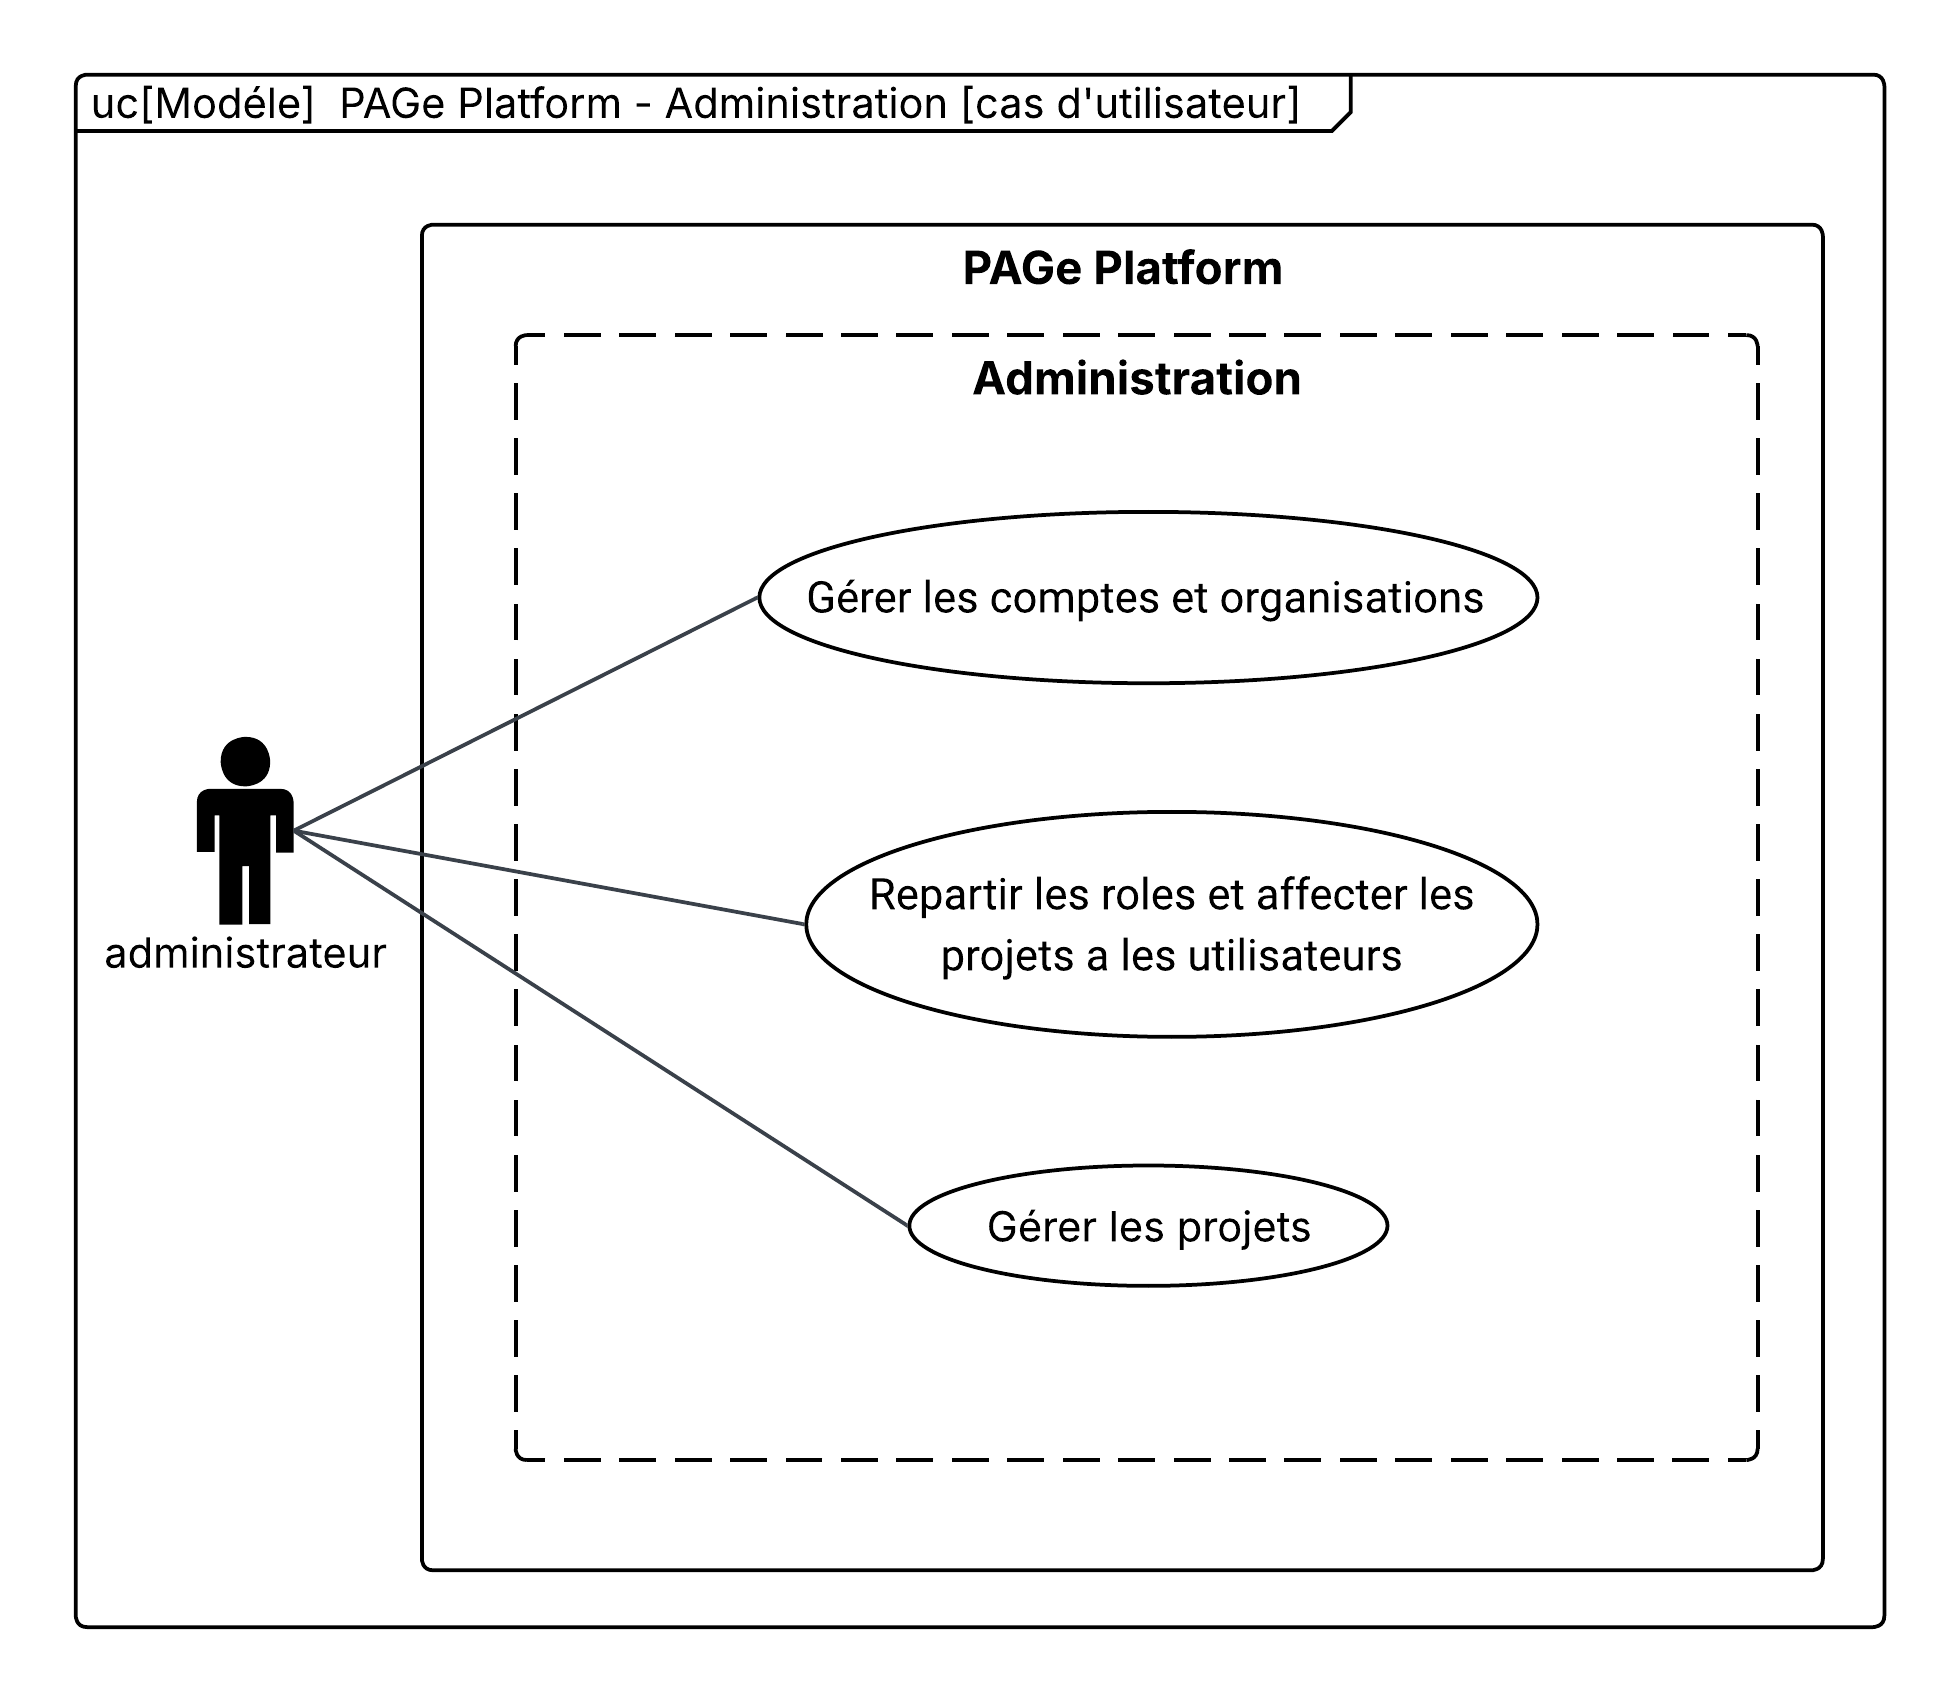
\includegraphics[width=0.9\textwidth]{figures/administration.png}
\caption{Diagramme de cas d'utilisation -- Administration}
\end{figure}

\subsubsection{Gérer les comptes et organisations}
\begin{table}[H]
\centering
\renewcommand{\arraystretch}{1.3}
\begin{tabular}{@{}p{0.25\textwidth}p{0.67\textwidth}@{}}
\hline
\multicolumn{2}{c}{\textbf{Sommaire d'identification}} \\
\hline
\textbf{Titre} & Gérer les comptes et organisations \\
\textbf{Objectif} & Créer, modifier et supprimer des comptes utilisateurs. \\
\textbf{Acteurs} & Administrateur \\
\hline
\multicolumn{2}{c}{\textbf{Description des scénarios}} \\
\hline
\textbf{Pré-conditions} & L'administrateur est authentifié. \\
\textbf{Scénario nominal} & L'administrateur accède à la page de gestion des comptes, crée un nouveau compte en renseignant le nom d'utilisateur, l'email et le mot de passe (généré automatiquement), puis attribue un rôle et affecte l'utilisateur à un projet. \\
\textbf{Scénarios secondaires} & Modifier un compte ; supprimer un compte ; consulter la liste des utilisateurs par projet. \\
\hline
\end{tabular}
\caption{Description -- Gérer les comptes}
\end{table}

\subsubsection{Répartir les rôles et affecter les projets aux utilisateurs}
\begin{table}[H]
\centering
\renewcommand{\arraystretch}{1.3}
\begin{tabular}{@{}p{0.25\textwidth}p{0.67\textwidth}@{}}
\hline
\multicolumn{2}{c}{\textbf{Sommaire d'identification}} \\
\hline
\textbf{Titre} & Répartir les rôles et affecter les projets aux utilisateurs \\
\textbf{Objectif} & Attribuer à chaque utilisateur son rôle et le projet auquel il appartient. \\
\textbf{Acteurs} & Administrateur \\
\hline
\multicolumn{2}{c}{\textbf{Description des scénarios}} \\
\hline
\textbf{Pré-conditions} & L'utilisateur cible existe ; au moins un projet est créé. \\
\textbf{Scénario nominal} & L'administrateur sélectionne un utilisateur, lui attribue un rôle parmi les six disponibles, et l'affecte à un projet existant. L'utilisateur ne verra que les données de son projet. \\
\textbf{Scénarios secondaires} & Modifier le rôle d'un utilisateur ; changer l'affectation de projet d'un utilisateur. \\
\hline
\end{tabular}
\caption{Description -- Répartir les rôles et affecter les projets}
\end{table}

\subsubsection{Gérer les projets}
\begin{table}[H]
\centering
\renewcommand{\arraystretch}{1.3}
\begin{tabular}{@{}p{0.25\textwidth}p{0.67\textwidth}@{}}
\hline
\multicolumn{2}{c}{\textbf{Sommaire d'identification}} \\
\hline
\textbf{Titre} & Gérer les projets \\
\textbf{Objectif} & Créer, modifier, activer/désactiver et supprimer des projets. Chaque projet représente un espace de travail indépendant avec ses propres données. \\
\textbf{Acteurs} & Administrateur \\
\hline
\multicolumn{2}{c}{\textbf{Description des scénarios}} \\
\hline
\textbf{Pré-conditions} & L'administrateur est authentifié. \\
\textbf{Scénario nominal} & L'administrateur crée un nouveau projet en renseignant un nom et une description. Le projet devient disponible pour l'affectation des utilisateurs. Toutes les données (risques, campagnes, mécanismes, simulations) créées au sein d'un projet sont isolées des autres projets. \\
\textbf{Scénarios secondaires} & Modifier le nom ou la description ; désactiver un projet ; supprimer un projet. \\
\hline
\end{tabular}
\caption{Description -- Gérer les projets}
\end{table}

\subsection{Module O-PAGe}

\begin{figure}[H]
\centering
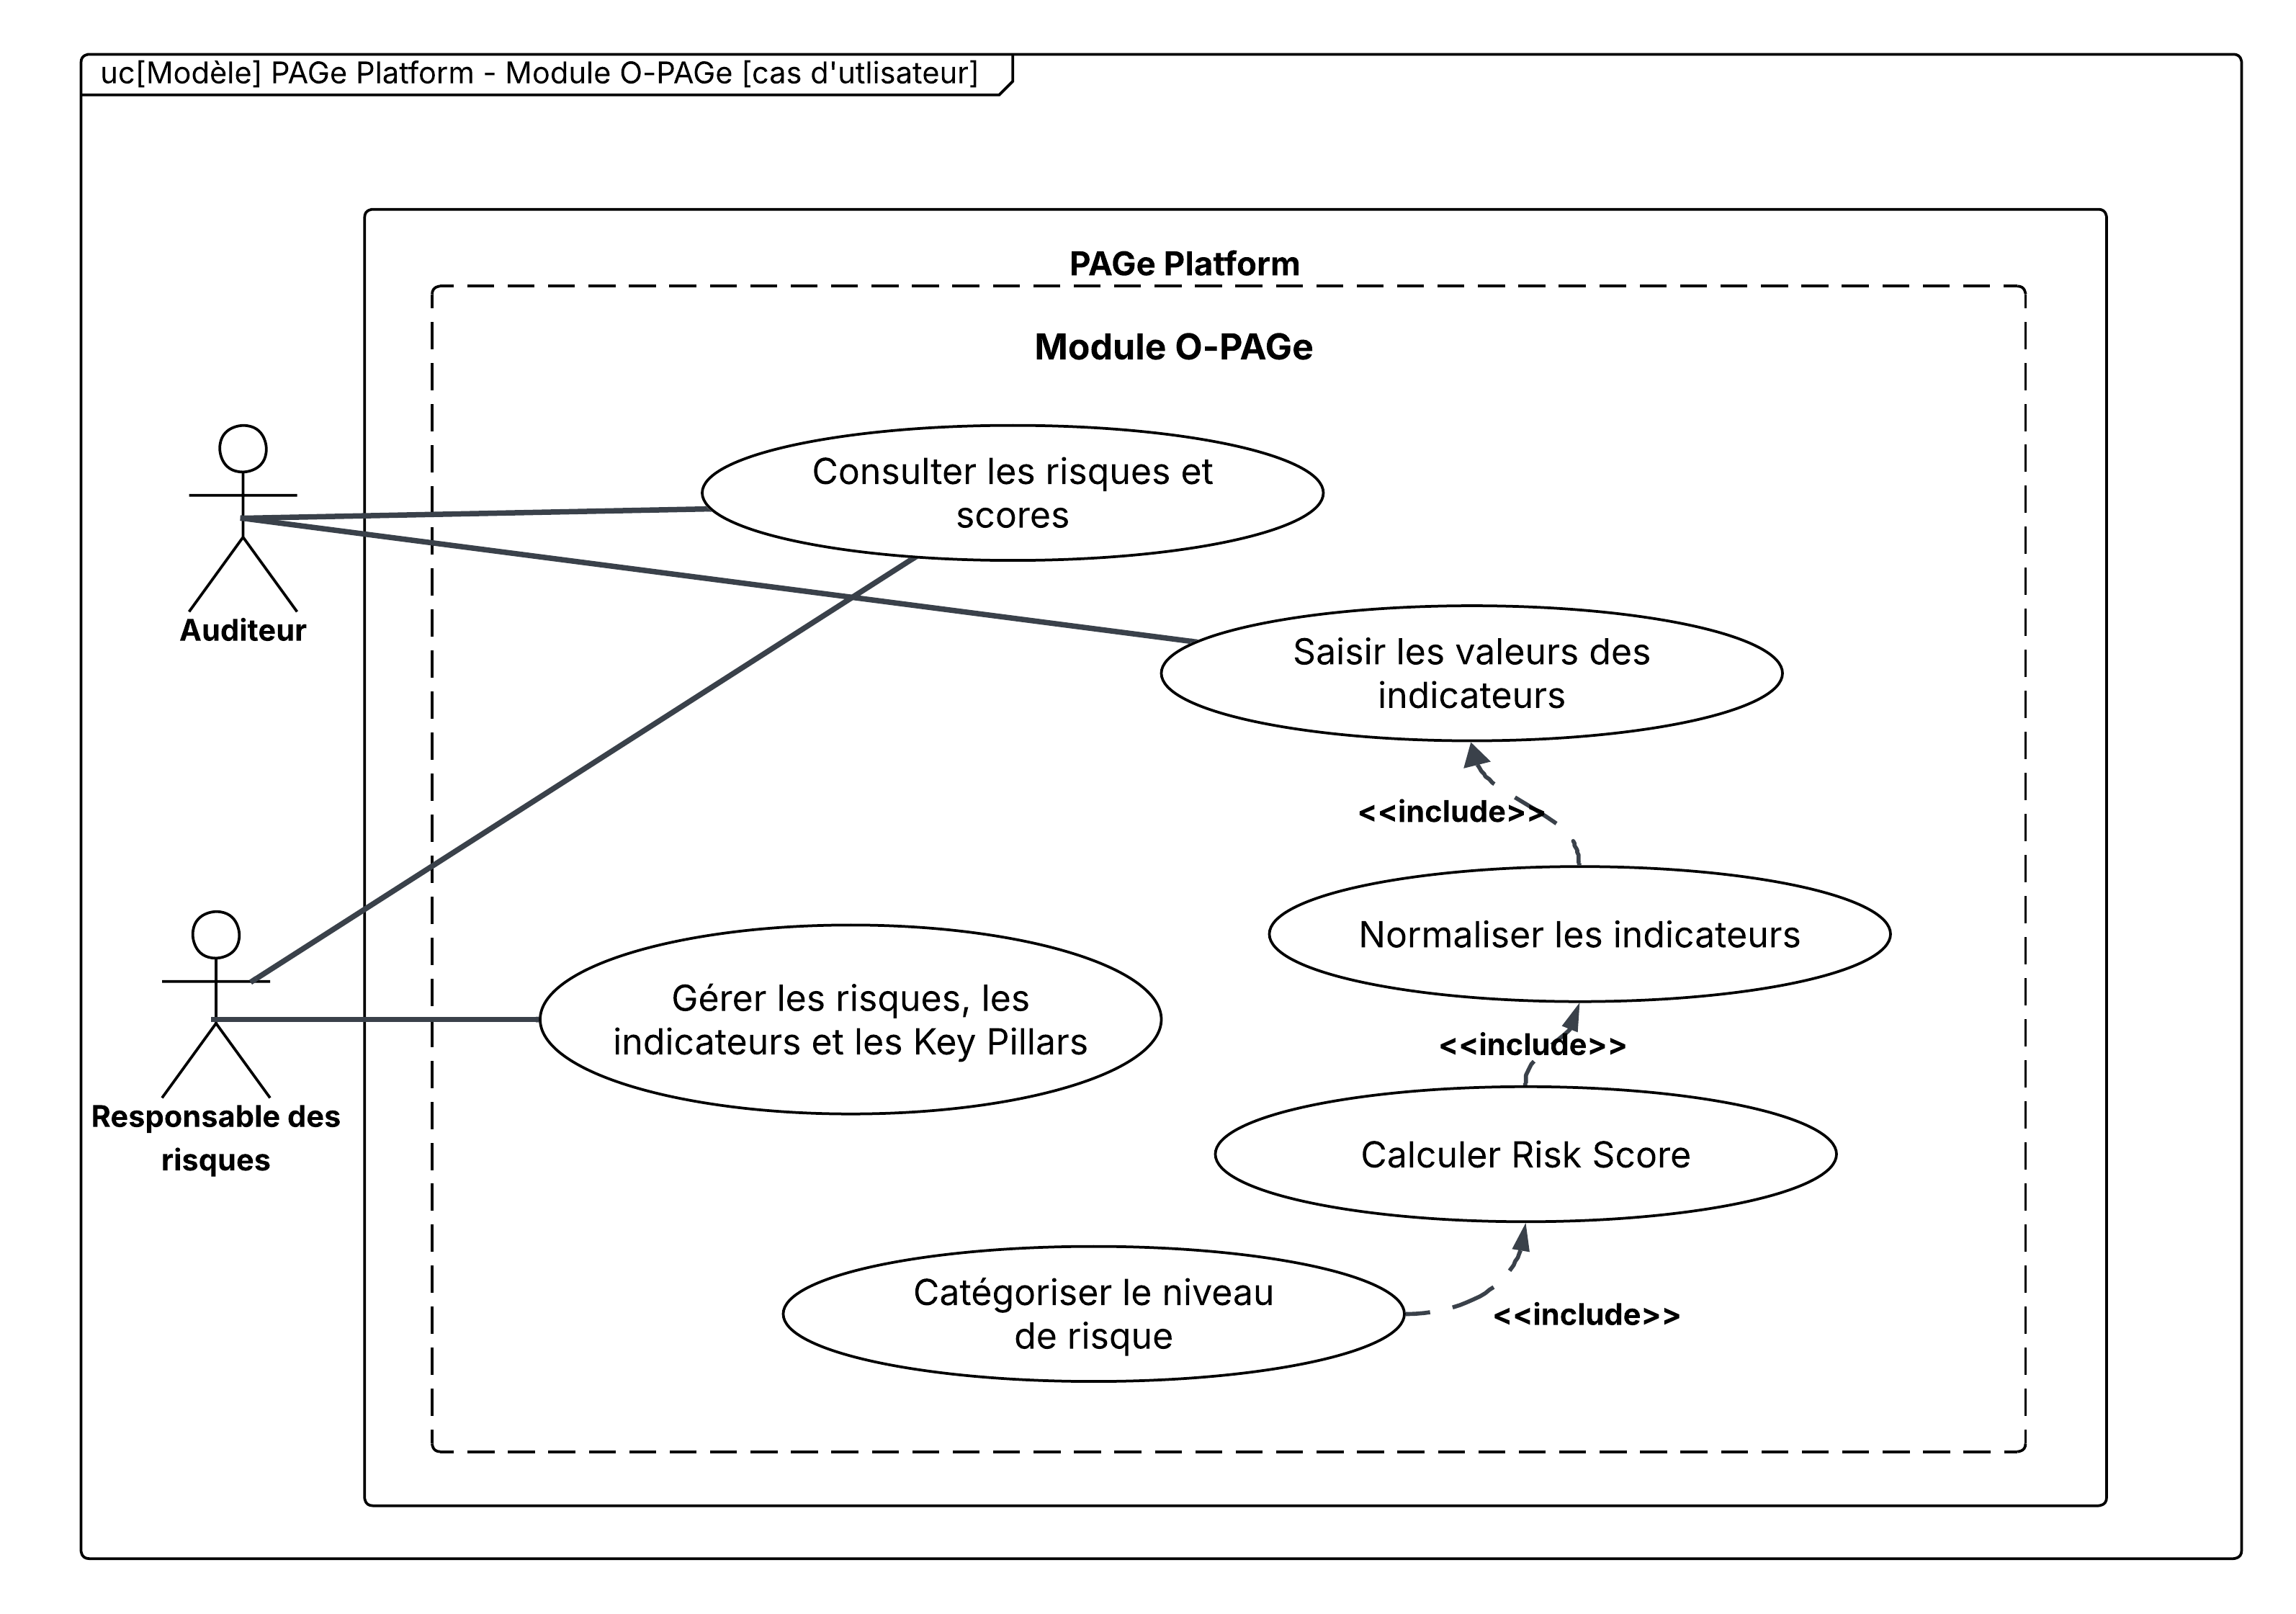
\includegraphics[width=0.85\textwidth]{figures/O-PAGe.png}
\caption{Diagramme de cas d'utilisation -- Module O-PAGe}
\end{figure}

\subsubsection{Gérer le modèle de risque et ses composants}
\begin{table}[H]
\centering
\renewcommand{\arraystretch}{1.3}
\begin{tabular}{@{}p{0.25\textwidth}p{0.67\textwidth}@{}}
\hline
\multicolumn{2}{c}{\textbf{Sommaire d'identification}} \\
\hline
\textbf{Titre} & Gérer le modèle de risque et ses composants \\
\textbf{Objectif} & Créer, modifier et supprimer des risques, leurs indicateurs et les Key Pillars. \\
\textbf{Acteurs} & Risk Manager \\
\hline
\multicolumn{2}{c}{\textbf{Description des scénarios}} \\
\hline
\textbf{Pré-conditions} & Authentifié avec le rôle Risk Manager. \\
\textbf{Scénario nominal} & Le Risk Manager crée un risque, lui associe des indicateurs (libellé, poids, statut, plage de valeurs) et gère les Key Pillars (nom, type). \\
\textbf{Scénarios secondaires} & Modifier un risque ; supprimer un indicateur ; ajuster les poids ; ajouter/supprimer un Key Pillar. \\
\hline
\end{tabular}
\caption{Description -- Gérer le modèle de risque}
\end{table}

\subsubsection{Saisir les valeurs des indicateurs}
\begin{table}[H]
\centering
\renewcommand{\arraystretch}{1.3}
\begin{tabular}{@{}p{0.25\textwidth}p{0.67\textwidth}@{}}
\hline
\multicolumn{2}{c}{\textbf{Sommaire d'identification}} \\
\hline
\textbf{Titre} & Saisir les valeurs des indicateurs \\
\textbf{Objectif} & Renseigner la valeur brute d'un indicateur. \\
\textbf{Acteurs} & Auditeur \\
\hline
\multicolumn{2}{c}{\textbf{Description des scénarios}} \\
\hline
\textbf{Pré-conditions} & Le risque et ses indicateurs existent. \\
\textbf{Scénario nominal} & L'auditeur sélectionne un risque, choisit un indicateur et saisit sa valeur. Le système calcule la valeur normalisée et déclenche le recalcul du Risk Score. \\
\textbf{Scénarios secondaires} & Modifier une valeur existante. \\
\hline
\end{tabular}
\caption{Description -- Saisir les valeurs des indicateurs}
\end{table}

\subsubsection{Calculer le Risk Score}
\begin{table}[H]
\centering
\renewcommand{\arraystretch}{1.3}
\begin{tabular}{@{}p{0.25\textwidth}p{0.67\textwidth}@{}}
\hline
\multicolumn{2}{c}{\textbf{Sommaire d'identification}} \\
\hline
\textbf{Titre} & Calculer le Risk Score \\
\textbf{Objectif} & Calculer automatiquement le score de gravité d'un risque. \\
\textbf{Acteurs} & Système (déclenché automatiquement) \\
\hline
\multicolumn{2}{c}{\textbf{Description des scénarios}} \\
\hline
\textbf{Pré-conditions} & Au moins un indicateur a une valeur saisie. \\
\textbf{Scénario nominal} & Après chaque saisie d'une valeur d'indicateur, le système normalise les valeurs, calcule la somme pondérée et catégorise le risque (Low/Moderate/High/Critical). \\
\textbf{Scénarios secondaires} & Recalcul après modification d'une valeur. \\
\hline
\end{tabular}
\caption{Description -- Calculer le Risk Score}
\end{table}

\subsubsection{Consulter les Risk Scores}
\begin{table}[H]
\centering
\renewcommand{\arraystretch}{1.3}
\begin{tabular}{@{}p{0.25\textwidth}p{0.67\textwidth}@{}}
\hline
\multicolumn{2}{c}{\textbf{Sommaire d'identification}} \\
\hline
\textbf{Titre} & Consulter les Risk Scores \\
\textbf{Objectif} & Visualiser les scores de risque et leur catégorisation. \\
\textbf{Acteurs} & Risk Manager, Auditeur \\
\hline
\multicolumn{2}{c}{\textbf{Description des scénarios}} \\
\hline
\textbf{Pré-conditions} & Au moins un Risk Score a été calculé. \\
\textbf{Scénario nominal} & L'utilisateur accède à la page des risques et consulte le score, la catégorie (Low/Moderate/High/Critical) et les statistiques associées. \\
\textbf{Scénarios secondaires} & Filtrer par catégorie de risque. \\
\hline
\end{tabular}
\caption{Description -- Consulter les Risk Scores}
\end{table}

\subsection{Module M-PAGe}

\begin{figure}[H]
\centering
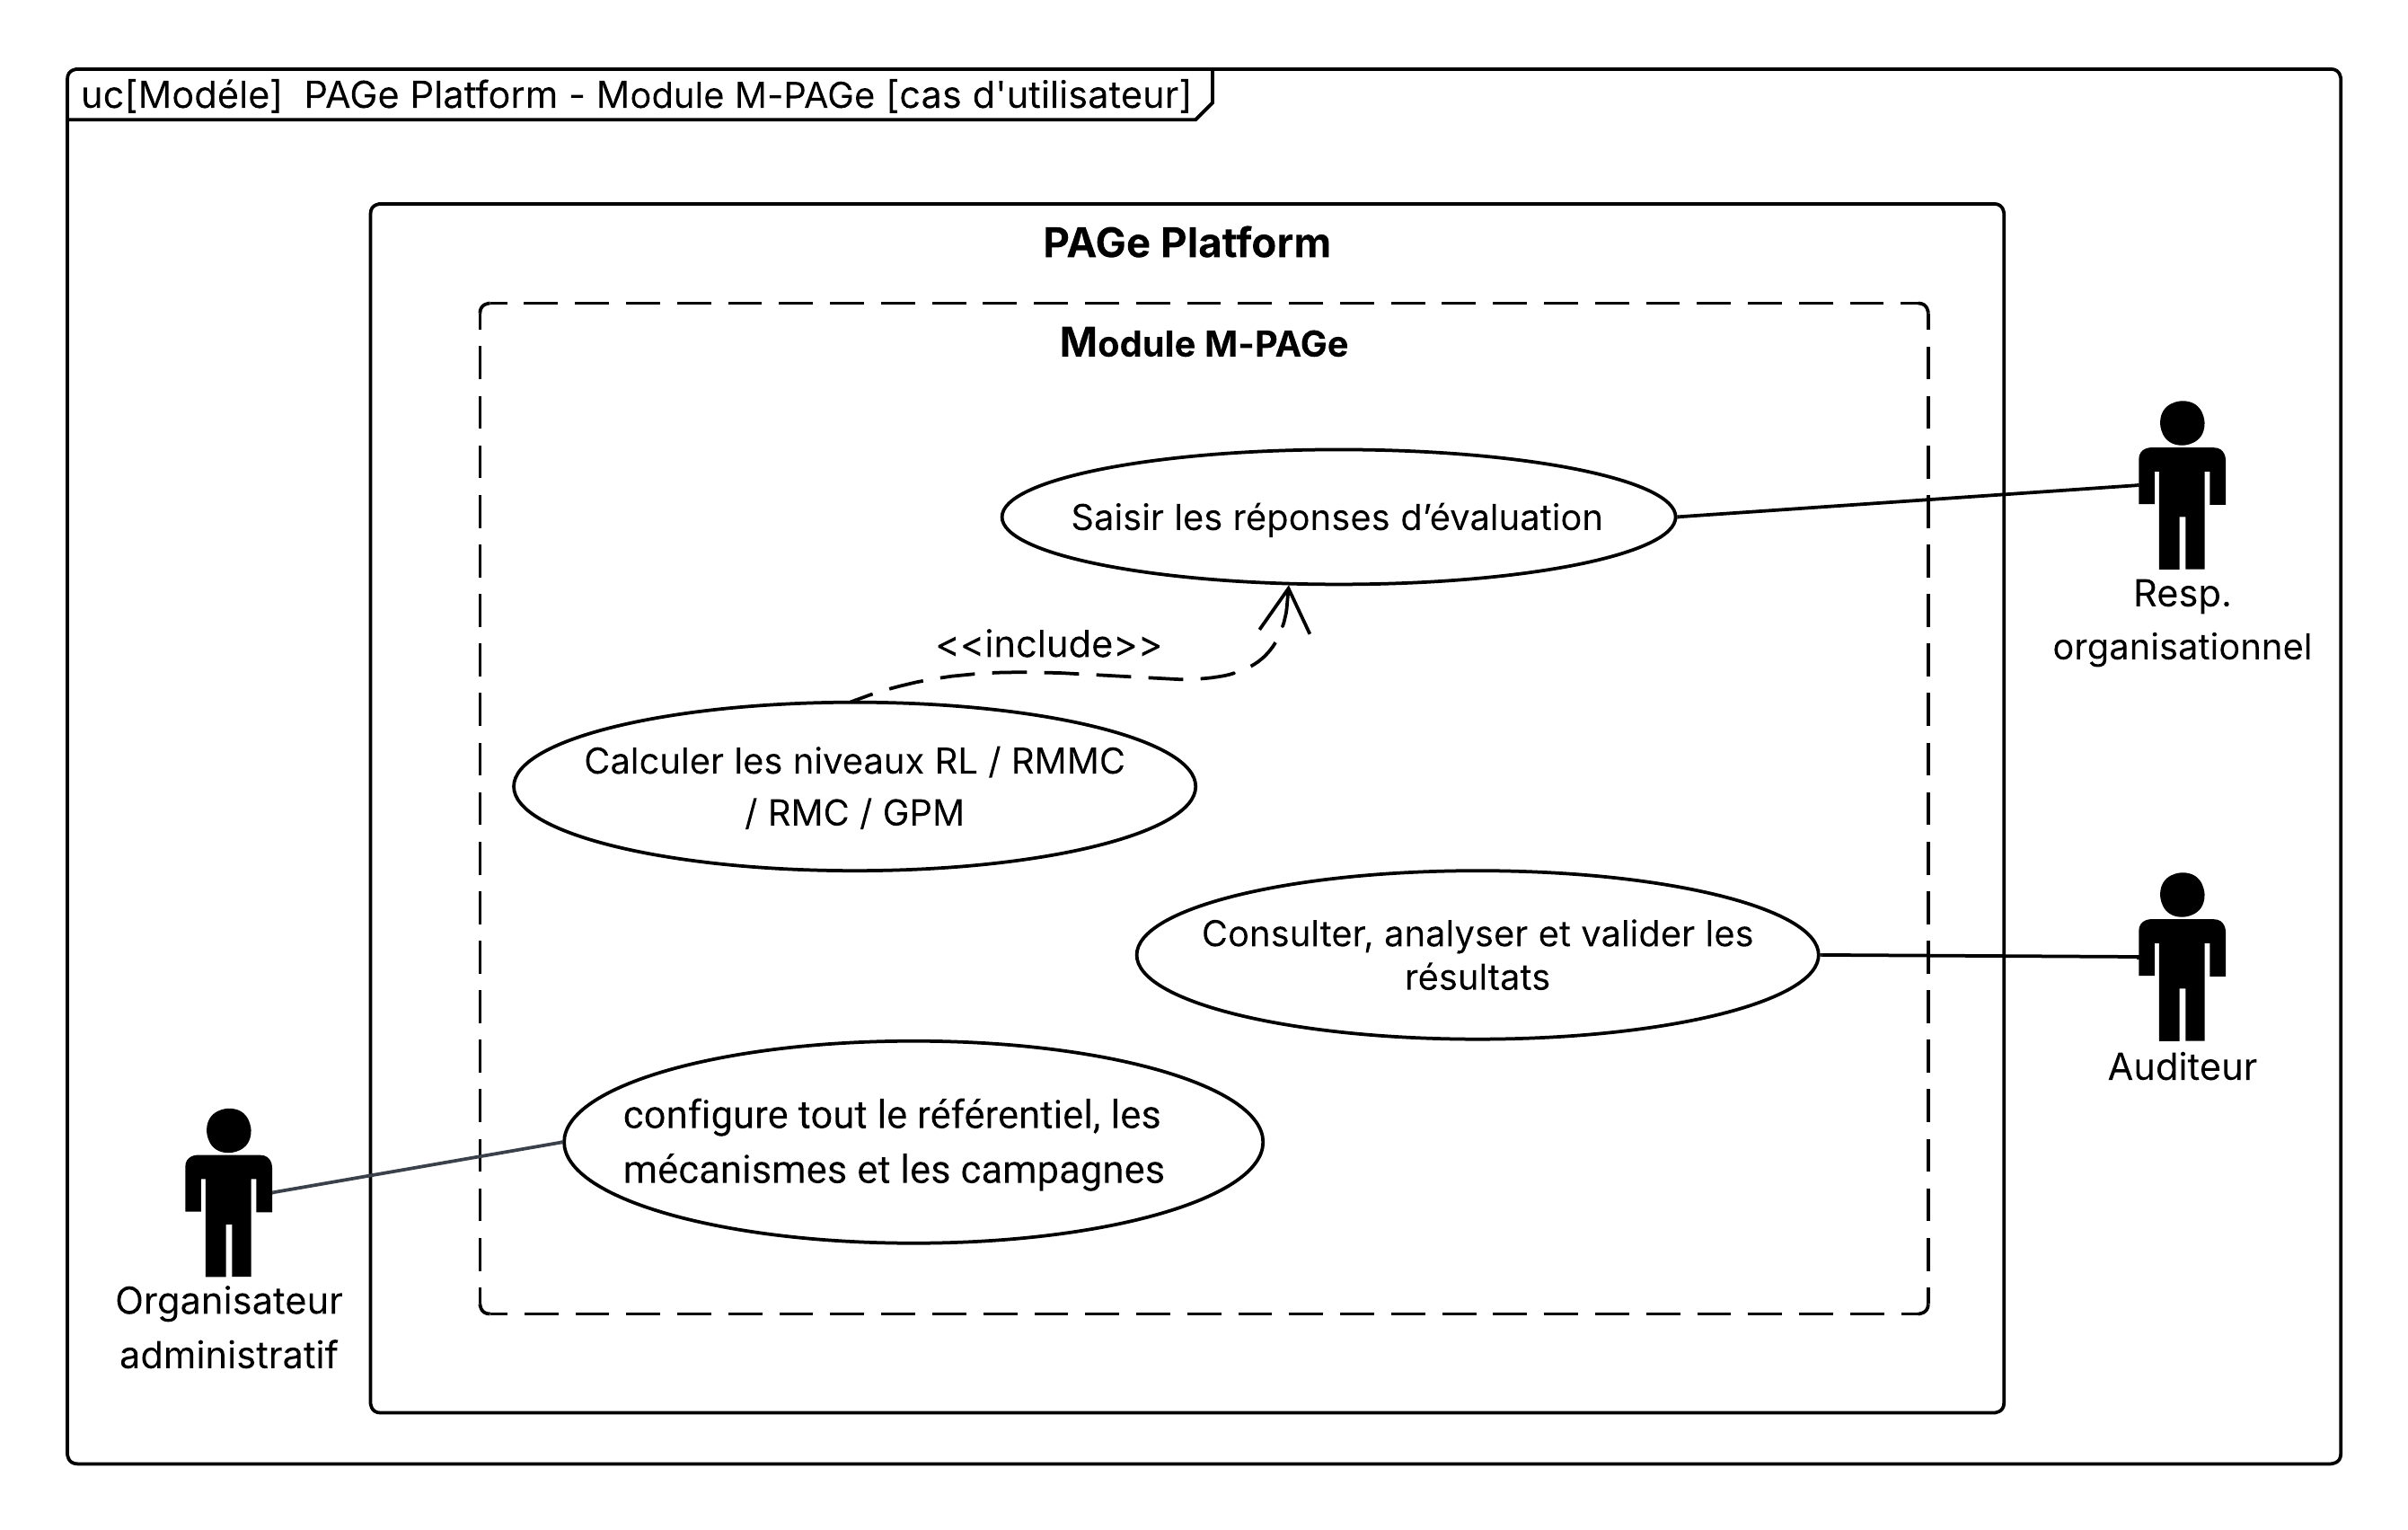
\includegraphics[width=1\textwidth]{figures/M-PAGe.png}
\caption{Diagramme de cas d'utilisation -- Module M-PAGe}
\end{figure}

\subsubsection{Gérer les poids des piliers/RMM}
\begin{table}[H]
\centering
\renewcommand{\arraystretch}{1.3}
\begin{tabular}{@{}p{0.25\textwidth}p{0.67\textwidth}@{}}
\hline
\multicolumn{2}{c}{\textbf{Sommaire d'identification}} \\
\hline
\textbf{Titre} & Gérer les poids des piliers/RMM \\
\textbf{Objectif} & Configurer les poids de chaque pilier dans un mécanisme. \\
\textbf{Acteurs} & Organisateur administratif \\
\hline
\multicolumn{2}{c}{\textbf{Description des scénarios}} \\
\hline
\textbf{Pré-conditions} & Mécanismes et piliers existent. \\
\textbf{Scénario nominal} & L'organisateur sélectionne un mécanisme, attribue un poids à chaque pilier (somme = 1), valide. \\
\textbf{Scénarios secondaires} & Modifier les poids existants. \\
\hline
\end{tabular}
\caption{Description -- Gérer les poids des piliers/RMM}
\end{table}

\subsubsection{Saisir les réponses d'évaluation}
\begin{table}[H]
\centering
\renewcommand{\arraystretch}{1.3}
\begin{tabular}{@{}p{0.25\textwidth}p{0.67\textwidth}@{}}
\hline
\multicolumn{2}{c}{\textbf{Sommaire d'identification}} \\
\hline
\textbf{Titre} & Saisir les réponses d'évaluation \\
\textbf{Objectif} & Répondre au questionnaire de maturité. \\
\textbf{Acteurs} & Responsable organisationnel \\
\hline
\multicolumn{2}{c}{\textbf{Description des scénarios}} \\
\hline
\textbf{Pré-conditions} & Campagne en cours. \\
\textbf{Scénario nominal} & Le responsable répond aux items (1 à 5) et soumet. \\
\textbf{Scénarios secondaires} & Modifier avant soumission. \\
\hline
\end{tabular}
\caption{Description -- Saisir les réponses d'évaluation}
\end{table}

\subsubsection{Consulter et valider les résultats}
\begin{table}[H]
\centering
\renewcommand{\arraystretch}{1.3}
\begin{tabular}{@{}p{0.25\textwidth}p{0.67\textwidth}@{}}
\hline
\multicolumn{2}{c}{\textbf{Sommaire d'identification}} \\
\hline
\textbf{Titre} & Consulter et valider les résultats \\
\textbf{Objectif} & Visualiser les scores RL, RMMC, RMC et GPM. \\
\textbf{Acteurs} & Auditeur \\
\hline
\multicolumn{2}{c}{\textbf{Description des scénarios}} \\
\hline
\textbf{Pré-conditions} & Campagne clôturée, scores calculés. \\
\textbf{Scénario nominal} & L'auditeur consulte les résultats par pilier et mécanisme. \\
\textbf{Scénarios secondaires} & Exporter ; comparer des campagnes. \\
\hline
\end{tabular}
\caption{Description -- Consulter et valider les résultats}
\end{table}

\subsection{Gestion des campagnes}

\begin{figure}[H]
\centering
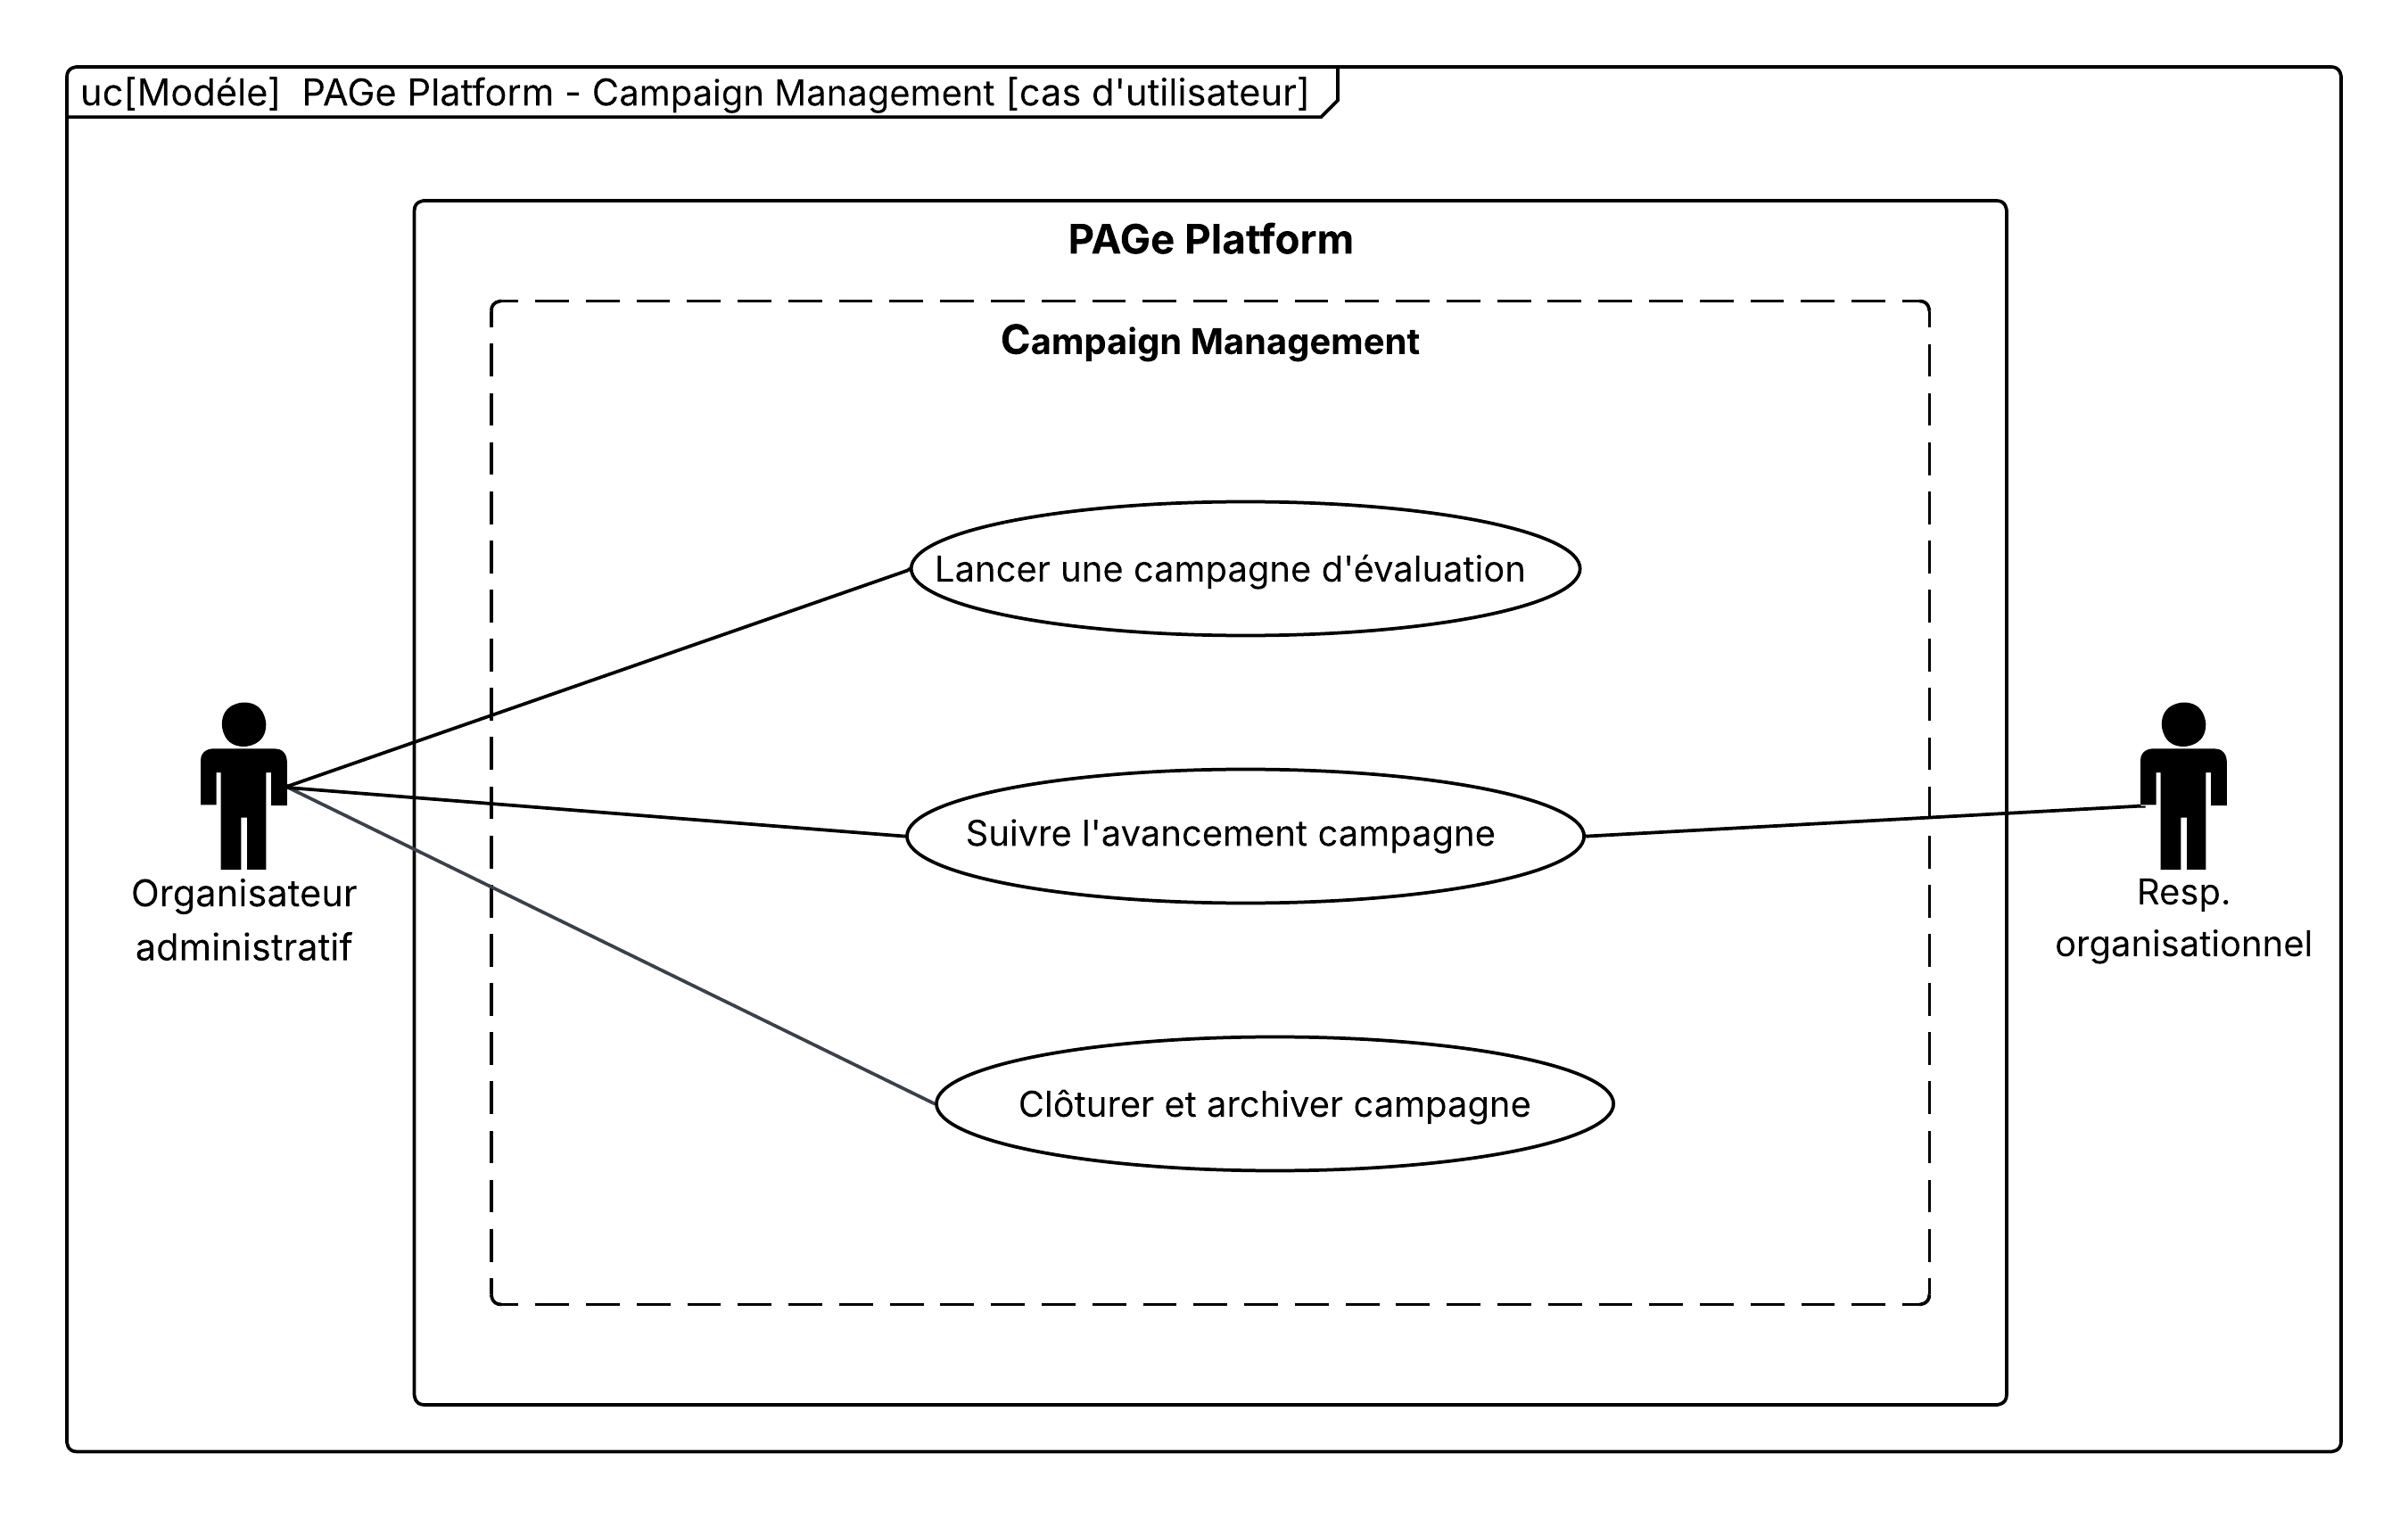
\includegraphics[width=0.90\textwidth]{figures/UC_Campaigns.png}
\caption{Diagramme de cas d'utilisation -- Gestion des campagnes}
\end{figure}

\subsubsection{Lancer une campagne}
\begin{table}[H]
\centering
\renewcommand{\arraystretch}{1.3}
\begin{tabular}{@{}p{0.25\textwidth}p{0.67\textwidth}@{}}
\hline
\multicolumn{2}{c}{\textbf{Sommaire d'identification}} \\
\hline
\textbf{Titre} & Lancer une campagne d'évaluation \\
\textbf{Objectif} & Créer et démarrer une campagne. \\
\textbf{Acteurs} & Organisateur administratif \\
\hline
\multicolumn{2}{c}{\textbf{Description des scénarios}} \\
\hline
\textbf{Pré-conditions} & Référentiel configuré. \\
\textbf{Scénario nominal} & L'organisateur crée une campagne, lui donne un nom, et la lance. \\
\textbf{Scénarios secondaires} & Suivre l'avancement ; clôturer. \\
\hline
\end{tabular}
\caption{Description -- Lancer une campagne}
\end{table}

\subsubsection{Suivre l'avancement}
\begin{table}[H]
\centering
\renewcommand{\arraystretch}{1.3}
\begin{tabular}{@{}p{0.25\textwidth}p{0.67\textwidth}@{}}
\hline
\multicolumn{2}{c}{\textbf{Sommaire d'identification}} \\
\hline
\textbf{Titre} & Suivre l'avancement \\
\textbf{Objectif} & Voir le taux de complétion. \\
\textbf{Acteurs} & Organisateur administratif, Responsable organisationnel \\
\hline
\multicolumn{2}{c}{\textbf{Description des scénarios}} \\
\hline
\textbf{Pré-conditions} & Campagne en cours. \\
\textbf{Scénario nominal} & L'utilisateur consulte le pourcentage d'avancement. \\
\textbf{Scénarios secondaires} & -- \\
\hline
\end{tabular}
\caption{Description -- Suivre l'avancement}
\end{table}

\subsection{Module I-PAGe}

\begin{figure}[H]
\centering
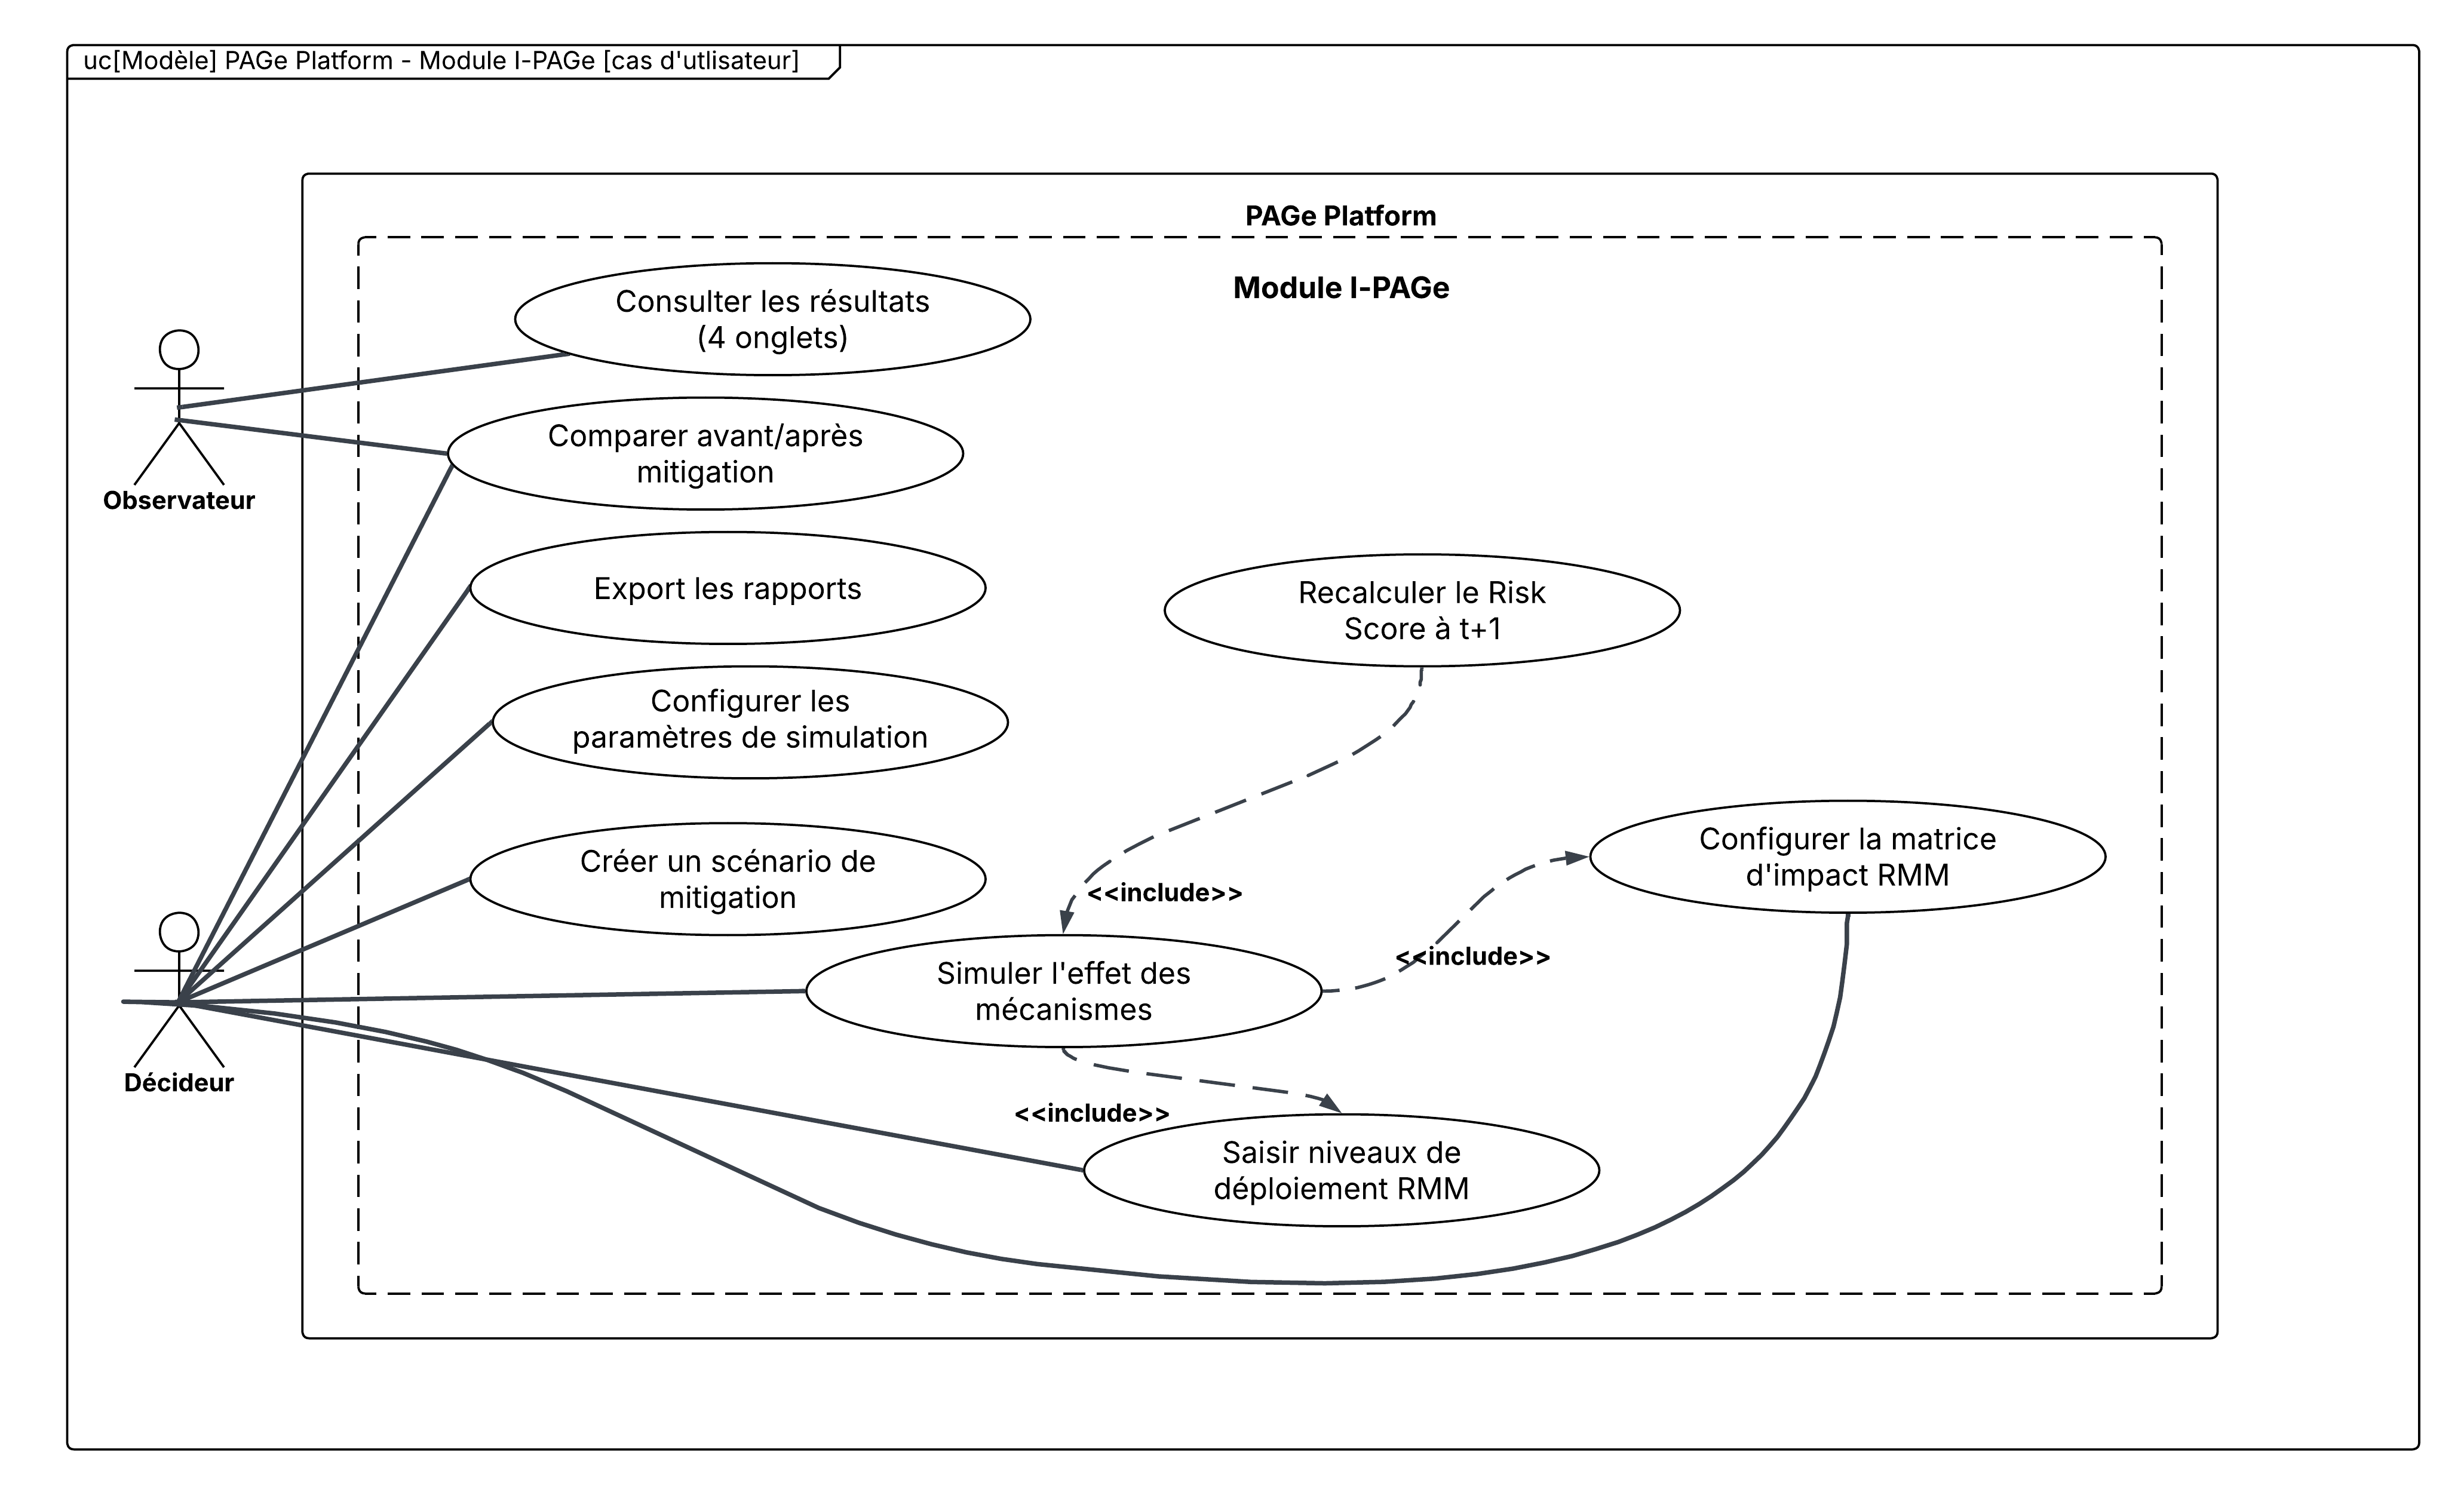
\includegraphics[width=0.85\textwidth]{figures/I-PAGe New.png}
\caption{Diagramme de cas d'utilisation -- Module I-PAGe}
\end{figure}

\subsubsection{Consulter les résultats}
\begin{table}[H]
\centering
\renewcommand{\arraystretch}{1.3}
\begin{tabular}{@{}p{0.25\textwidth}p{0.67\textwidth}@{}}
\hline
\multicolumn{2}{c}{\textbf{Sommaire d'identification}} \\
\hline
\textbf{Titre} & Consulter les résultats (4 onglets) \\
\textbf{Objectif} & Visualiser les résultats de simulation à travers les 4 étapes. \\
\textbf{Acteurs} & Observateur, Décideur \\
\hline
\multicolumn{2}{c}{\textbf{Description des scénarios}} \\
\hline
\textbf{Pré-conditions} & Une simulation a été exécutée. \\
\textbf{Scénario nominal} & L'utilisateur consulte les résultats via les onglets Paramètres, Simulation, Matrice d'impact et Résultats. \\
\textbf{Scénarios secondaires} & Aucun. \\
\hline
\end{tabular}
\caption{Description -- Consulter les résultats}
\end{table}

\subsubsection{Comparer avant/après mitigation}
\begin{table}[H]
\centering
\renewcommand{\arraystretch}{1.3}
\begin{tabular}{@{}p{0.25\textwidth}p{0.67\textwidth}@{}}
\hline
\multicolumn{2}{c}{\textbf{Sommaire d'identification}} \\
\hline
\textbf{Titre} & Comparer avant/après mitigation \\
\textbf{Objectif} & Comparer le Risk Score avant et après application des mécanismes. \\
\textbf{Acteurs} & Observateur, Décideur \\
\hline
\multicolumn{2}{c}{\textbf{Description des scénarios}} \\
\hline
\textbf{Pré-conditions} & Au moins une simulation exécutée. \\
\textbf{Scénario nominal} & L'utilisateur visualise la comparaison du score initial et du score post-simulation. \\
\textbf{Scénarios secondaires} & Comparer plusieurs scénarios entre eux. \\
\hline
\end{tabular}
\caption{Description -- Comparer avant/après mitigation}
\end{table}

\subsubsection{Exporter les rapports}
\begin{table}[H]
\centering
\renewcommand{\arraystretch}{1.3}
\begin{tabular}{@{}p{0.25\textwidth}p{0.67\textwidth}@{}}
\hline
\multicolumn{2}{c}{\textbf{Sommaire d'identification}} \\
\hline
\textbf{Titre} & Exporter les rapports \\
\textbf{Objectif} & Télécharger les résultats de simulation en PDF ou CSV. \\
\textbf{Acteurs} & Décideur \\
\hline
\multicolumn{2}{c}{\textbf{Description des scénarios}} \\
\hline
\textbf{Pré-conditions} & Des résultats de simulation disponibles. \\
\textbf{Scénario nominal} & Le décideur choisit le format (PDF/CSV) et lance l'export. \\
\textbf{Scénarios secondaires} & Sauvegarder les résultats en base. \\
\hline
\end{tabular}
\caption{Description -- Exporter les rapports}
\end{table}

\subsubsection{Configurer les paramètres de simulation}
\begin{table}[H]
\centering
\renewcommand{\arraystretch}{1.3}
\begin{tabular}{@{}p{0.25\textwidth}p{0.67\textwidth}@{}}
\hline
\multicolumn{2}{c}{\textbf{Sommaire d'identification}} \\
\hline
\textbf{Titre} & Configurer les paramètres de simulation \\
\textbf{Objectif} & Sélectionner les risques cibles et définir les paramètres. \\
\textbf{Acteurs} & Décideur \\
\hline
\multicolumn{2}{c}{\textbf{Description des scénarios}} \\
\hline
\textbf{Pré-conditions} & Des risques et indicateurs existent dans le système. \\
\textbf{Scénario nominal} & Le décideur sélectionne les risques et configure les paramètres de la simulation. \\
\textbf{Scénarios secondaires} & Modifier les paramètres existants. \\
\hline
\end{tabular}
\caption{Description -- Configurer les paramètres de simulation}
\end{table}

\subsubsection{Créer un scénario de mitigation}
\begin{table}[H]
\centering
\renewcommand{\arraystretch}{1.3}
\begin{tabular}{@{}p{0.25\textwidth}p{0.67\textwidth}@{}}
\hline
\multicolumn{2}{c}{\textbf{Sommaire d'identification}} \\
\hline
\textbf{Titre} & Créer un scénario de mitigation \\
\textbf{Objectif} & Définir un scénario en sélectionnant les mécanismes à appliquer. \\
\textbf{Acteurs} & Décideur \\
\hline
\multicolumn{2}{c}{\textbf{Description des scénarios}} \\
\hline
\textbf{Pré-conditions} & Des mécanismes RMM configurés. \\
\textbf{Scénario nominal} & Le décideur sélectionne les mécanismes et crée un scénario de mitigation. \\
\textbf{Scénarios secondaires} & Dupliquer un scénario existant. \\
\hline
\end{tabular}
\caption{Description -- Créer un scénario de mitigation}
\end{table}

\subsubsection{Simuler l'effet des mécanismes}
\begin{table}[H]
\centering
\renewcommand{\arraystretch}{1.3}
\begin{tabular}{@{}p{0.25\textwidth}p{0.67\textwidth}@{}}
\hline
\multicolumn{2}{c}{\textbf{Sommaire d'identification}} \\
\hline
\textbf{Titre} & Simuler l'effet des mécanismes \\
\textbf{Objectif} & Lancer la simulation d'impact des mécanismes sur le Risk Score. \\
\textbf{Acteurs} & Décideur \\
\hline
\multicolumn{2}{c}{\textbf{Description des scénarios}} \\
\hline
\textbf{Pré-conditions} & Scénario créé, matrice d'impact et niveaux de déploiement saisis. \\
\textbf{Scénario nominal} & Le décideur lance la simulation, le système recalcule les indicateurs à t+1 et affiche le nouveau Risk Score. \\
\textbf{Scénarios secondaires} & Comparer plusieurs scénarios ; sauvegarder les résultats. \\
\textbf{Inclut} & Configurer la matrice d'impact RMM ; Saisir niveaux de déploiement RMM. \\
\hline
\end{tabular}
\caption{Description -- Simuler l'effet des mécanismes}
\end{table}

\subsubsection{Configurer la matrice d'impact}
\begin{table}[H]
\centering
\renewcommand{\arraystretch}{1.3}
\begin{tabular}{@{}p{0.25\textwidth}p{0.67\textwidth}@{}}
\hline
\multicolumn{2}{c}{\textbf{Sommaire d'identification}} \\
\hline
\textbf{Titre} & Configurer la matrice d'impact RMM \\
\textbf{Objectif} & Définir les coefficients d'impact mécanisme/indicateur. \\
\textbf{Acteurs} & Décideur (via <<include>>) \\
\hline
\multicolumn{2}{c}{\textbf{Description des scénarios}} \\
\hline
\textbf{Pré-conditions} & Mécanismes et indicateurs existent. \\
\textbf{Scénario nominal} & Le décideur associe des indicateurs à un mécanisme et définit les valeurs d'impact. \\
\textbf{Scénarios secondaires} & Modifier des coefficients existants. \\
\hline
\end{tabular}
\caption{Description -- Configurer la matrice d'impact}
\end{table}

\subsubsection{Saisir niveaux de déploiement RMM}
\begin{table}[H]
\centering
\renewcommand{\arraystretch}{1.3}
\begin{tabular}{@{}p{0.25\textwidth}p{0.67\textwidth}@{}}
\hline
\multicolumn{2}{c}{\textbf{Sommaire d'identification}} \\
\hline
\textbf{Titre} & Saisir niveaux de déploiement RMM \\
\textbf{Objectif} & Définir le niveau de déploiement de chaque mécanisme dans le scénario. \\
\textbf{Acteurs} & Décideur (via <<include>>) \\
\hline
\multicolumn{2}{c}{\textbf{Description des scénarios}} \\
\hline
\textbf{Pré-conditions} & Scénario et RMM sélectionnés. \\
\textbf{Scénario nominal} & Le décideur définit le pourcentage de déploiement (0--100\%) pour chaque mécanisme. \\
\textbf{Scénarios secondaires} & Ajuster les niveaux après un premier calcul. \\
\hline
\end{tabular}
\caption{Description -- Saisir niveaux de déploiement RMM}
\end{table}

\subsection{Analytics et Reporting}

\begin{figure}[H]
\centering
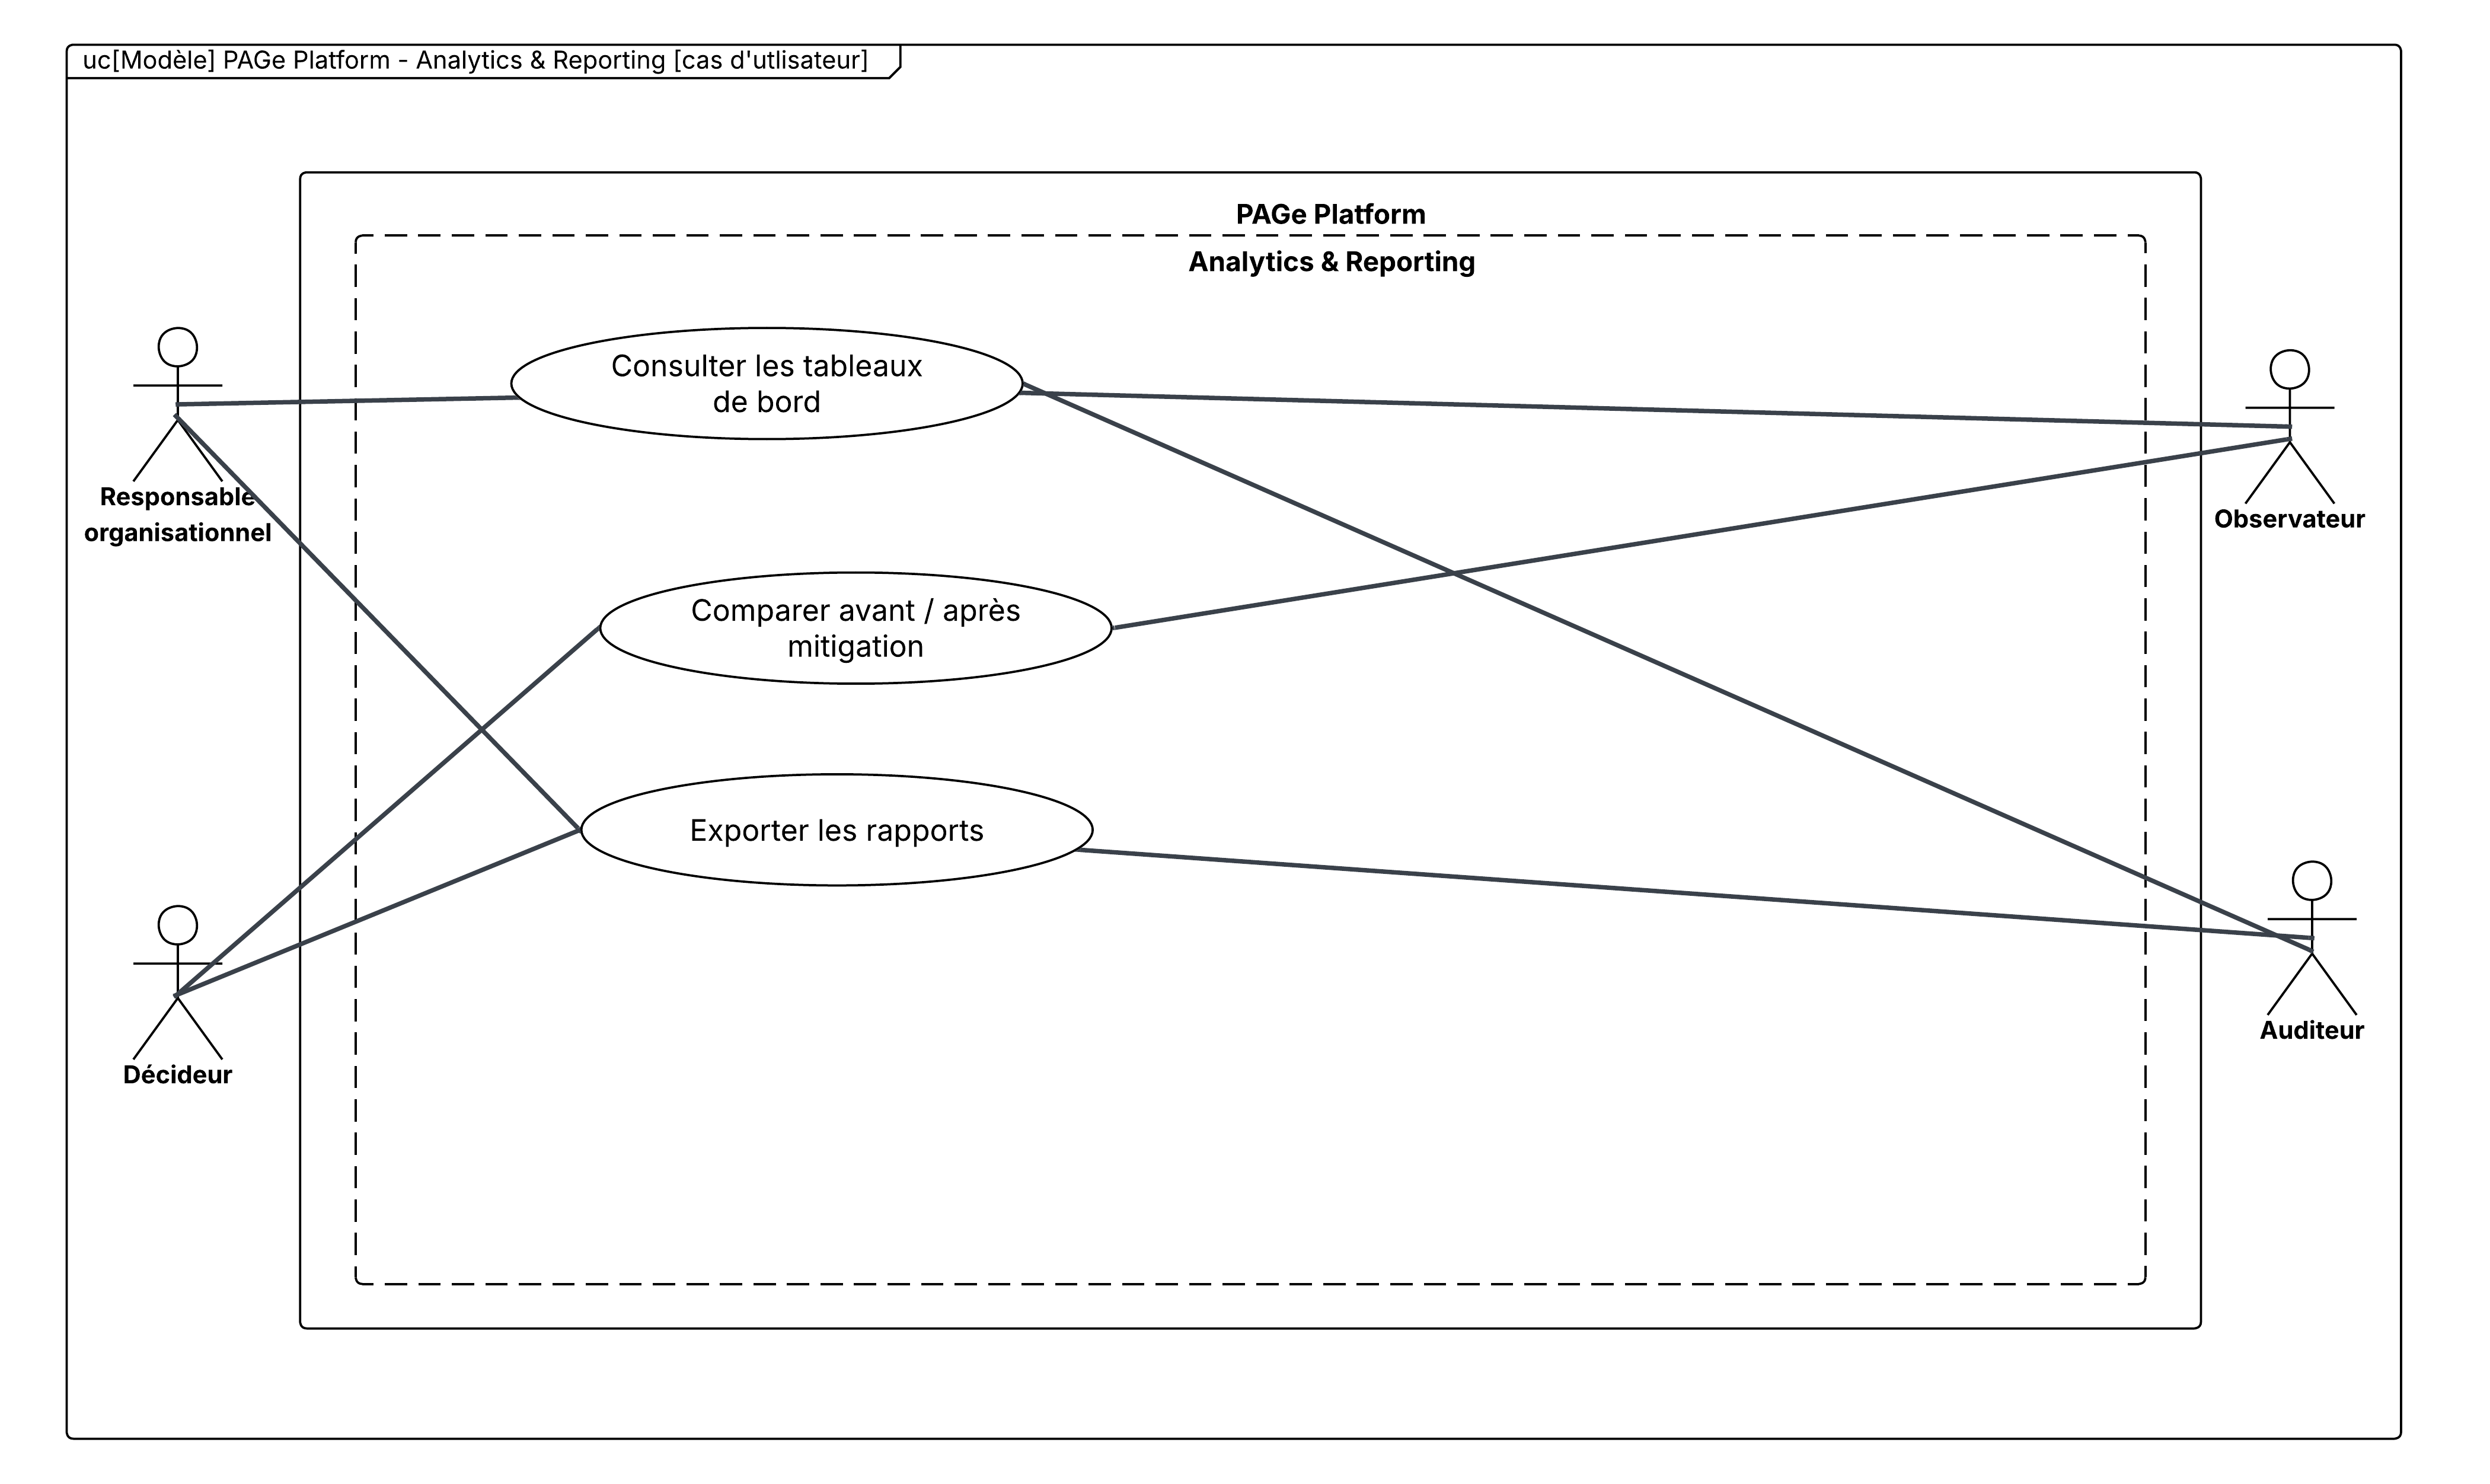
\includegraphics[width=0.85\textwidth]{figures/Analytics and Reporting.png}
\caption{Diagramme de cas d'utilisation -- Analytics et Reporting}
\end{figure}

\subsubsection{Consulter les tableaux de bord}
\begin{table}[H]
\centering
\renewcommand{\arraystretch}{1.3}
\begin{tabular}{@{}p{0.25\textwidth}p{0.67\textwidth}@{}}
\hline
\multicolumn{2}{c}{\textbf{Sommaire d'identification}} \\
\hline
\textbf{Titre} & Consulter les tableaux de bord \\
\textbf{Objectif} & Visualiser les résultats globaux. \\
\textbf{Acteurs} & Responsable organisationnel, Observateur, Auditeur \\
\hline
\multicolumn{2}{c}{\textbf{Description des scénarios}} \\
\hline
\textbf{Pré-conditions} & Des résultats existent. \\
\textbf{Scénario nominal} & L'utilisateur visualise les scores par risque, par mécanisme et le GPM global. \\
\textbf{Scénarios secondaires} & Filtrer par campagne. \\
\hline
\end{tabular}
\caption{Description -- Consulter les tableaux de bord}
\end{table}

\subsubsection{Comparer avant/après mitigation}
\begin{table}[H]
\centering
\renewcommand{\arraystretch}{1.3}
\begin{tabular}{@{}p{0.25\textwidth}p{0.67\textwidth}@{}}
\hline
\multicolumn{2}{c}{\textbf{Sommaire d'identification}} \\
\hline
\textbf{Titre} & Comparer avant/après mitigation \\
\textbf{Objectif} & Analyser l'évolution des scores entre campagnes ou avant/après simulation. \\
\textbf{Acteurs} & Décideur, Observateur, Auditeur \\
\hline
\multicolumn{2}{c}{\textbf{Description des scénarios}} \\
\hline
\textbf{Pré-conditions} & Au moins deux jeux de résultats disponibles. \\
\textbf{Scénario nominal} & L'utilisateur sélectionne les éléments à comparer et visualise les écarts. \\
\textbf{Scénarios secondaires} & Comparer plusieurs campagnes entre elles. \\
\hline
\end{tabular}
\caption{Description -- Comparer avant/après mitigation}
\end{table}

\subsubsection{Exporter les rapports}
\begin{table}[H]
\centering
\renewcommand{\arraystretch}{1.3}
\begin{tabular}{@{}p{0.25\textwidth}p{0.67\textwidth}@{}}
\hline
\multicolumn{2}{c}{\textbf{Sommaire d'identification}} \\
\hline
\textbf{Titre} & Exporter les rapports \\
\textbf{Objectif} & Télécharger un rapport PDF ou Excel. \\
\textbf{Acteurs} & Responsable organisationnel, Décideur, Auditeur \\
\hline
\multicolumn{2}{c}{\textbf{Description des scénarios}} \\
\hline
\textbf{Pré-conditions} & Des résultats existent. \\
\textbf{Scénario nominal} & L'utilisateur choisit le format et lance l'export. \\
\textbf{Scénarios secondaires} & Choisir les données à inclure. \\
\hline
\end{tabular}
\caption{Description -- Exporter les rapports}
\end{table}

\section{Diagramme de classes}

\begin{figure}[H]
\centering
\makebox[\textwidth]{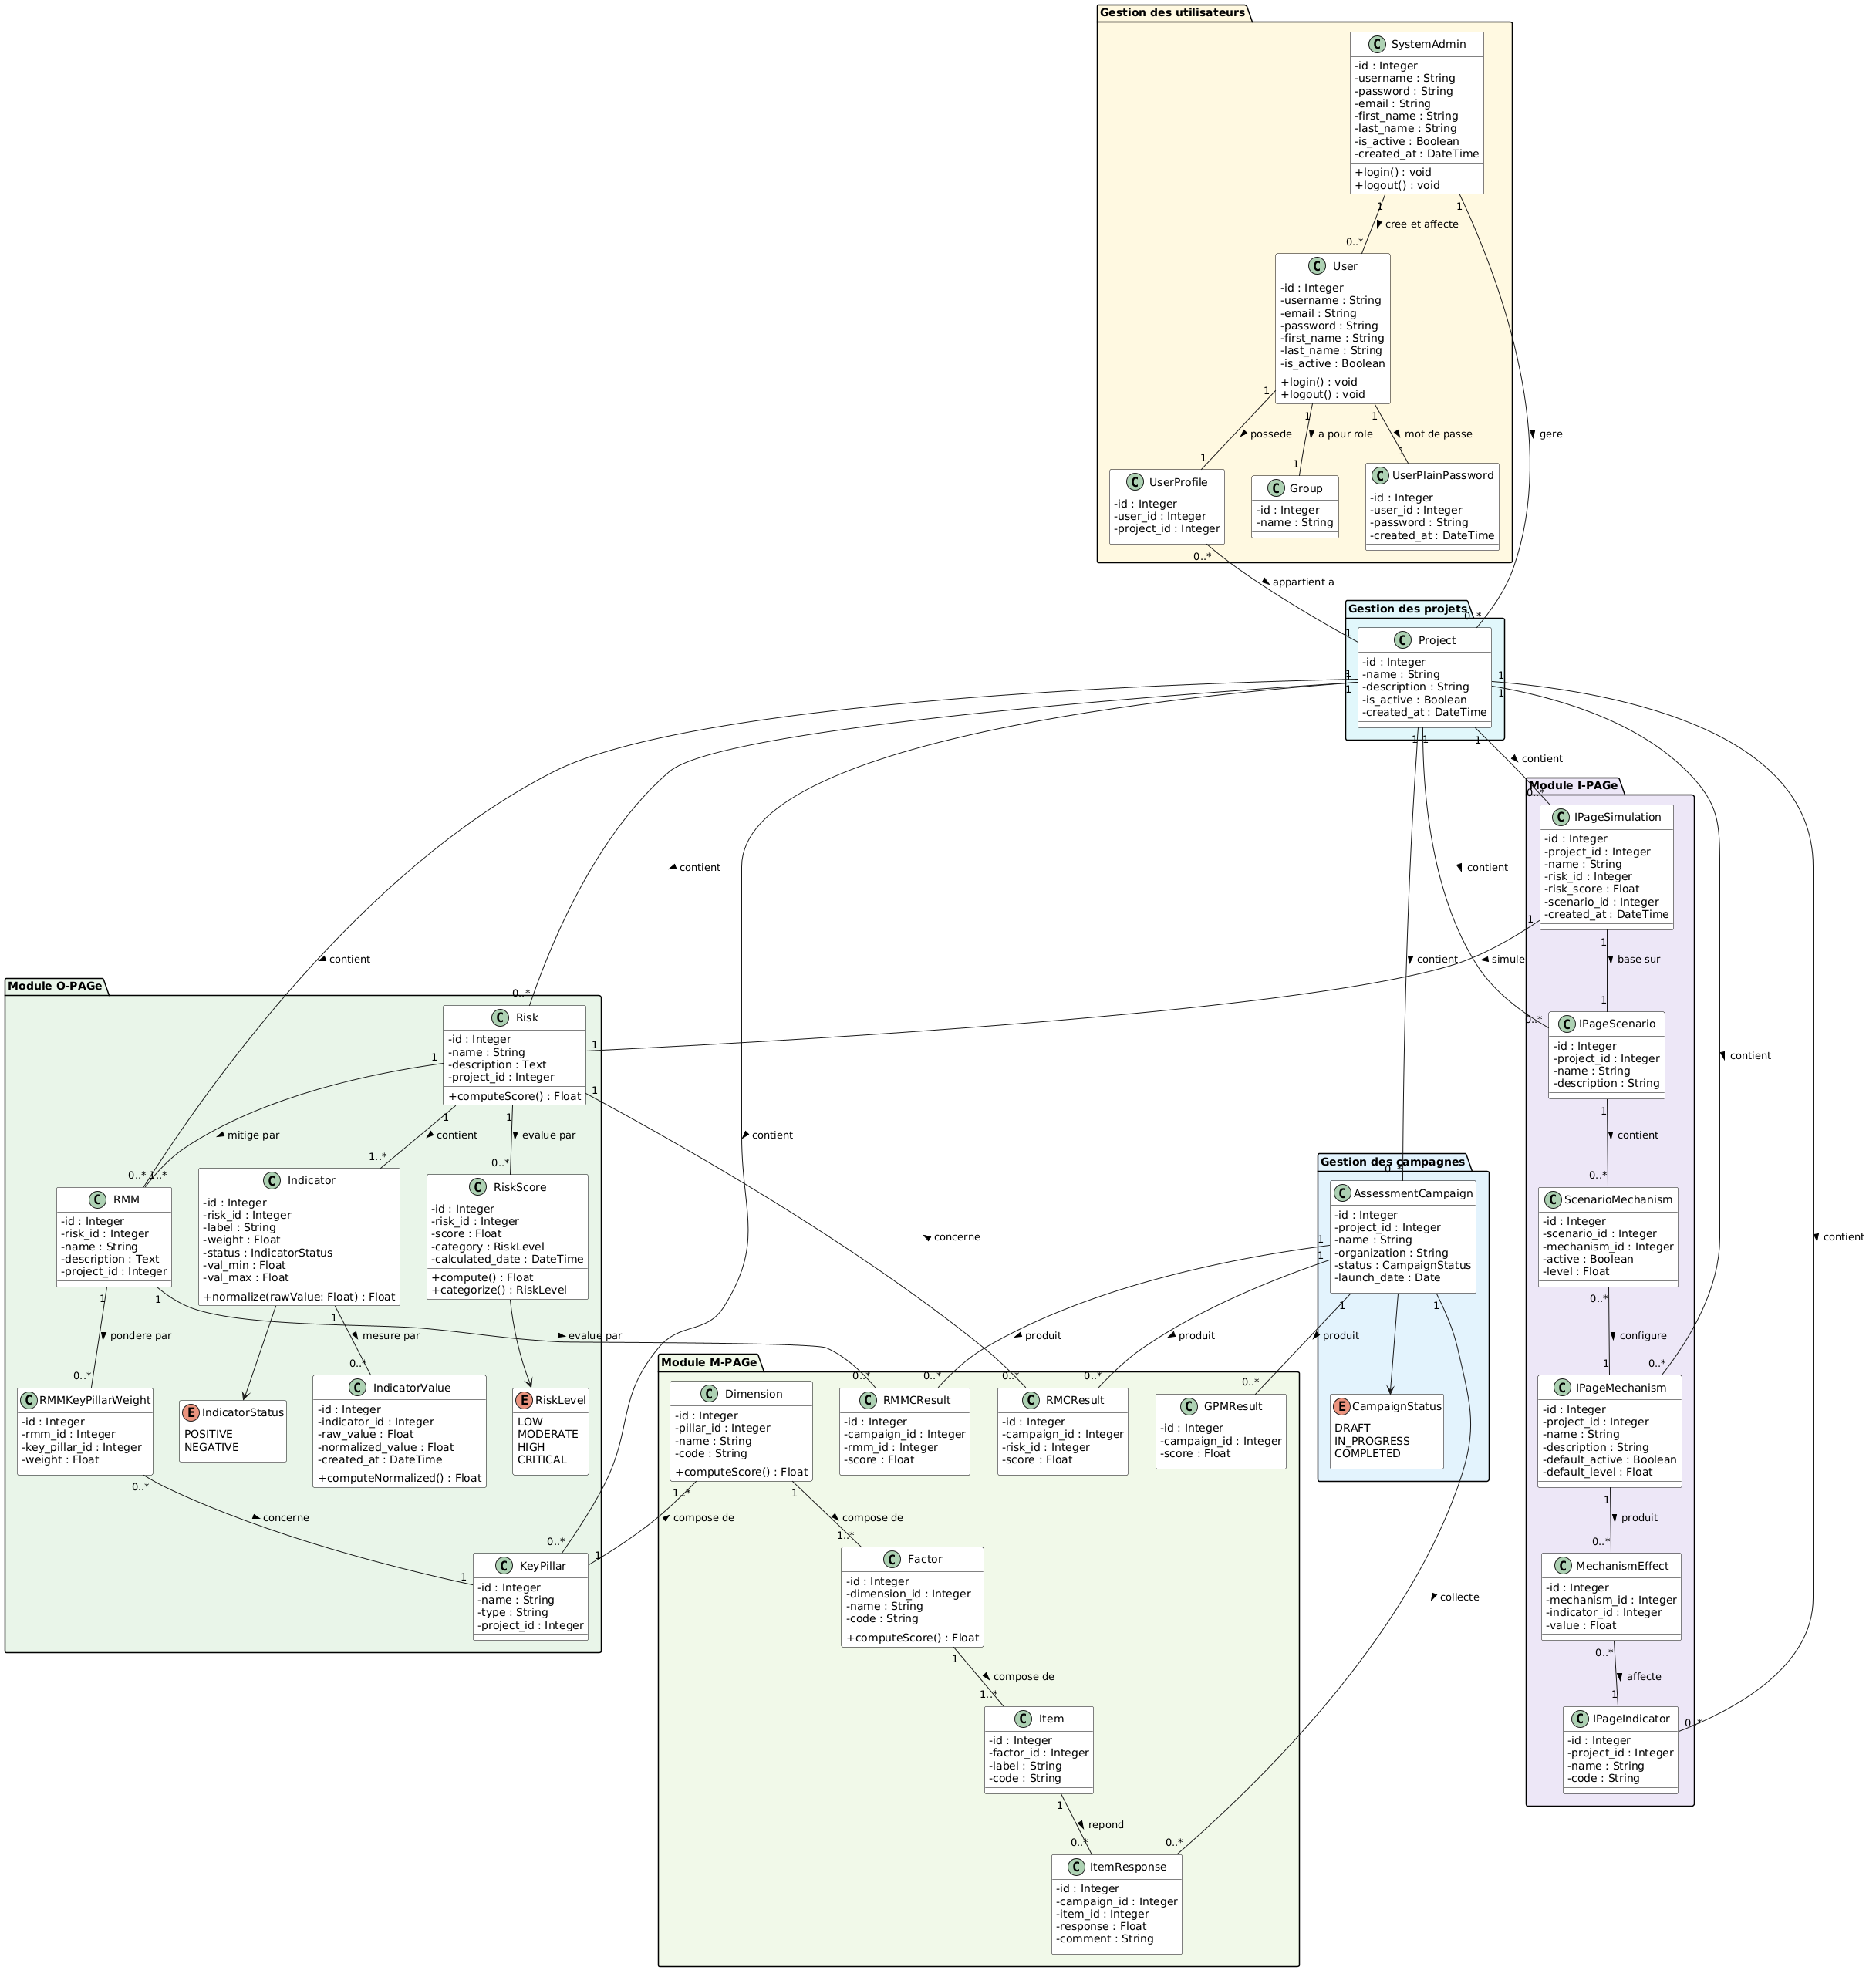
\includegraphics[width=1.2\textwidth]{figures/class_diagram.png}}
\caption{Diagramme de classes de la PAGe Platform}
\end{figure}

Les classes sont regroupées en six packages :
\begin{itemize}
    \item \textbf{Gestion des utilisateurs} : SystemAdmin, User, UserProfile, Group, UserPlainPassword
    \item \textbf{Gestion des projets} : Project
    \item \textbf{Module O-PAGe} : Risk, RiskScore, Indicator, IndicatorValue, KeyPillar, RMM, RMMKeyPillarWeight
    \item \textbf{Gestion des campagnes} : AssessmentCampaign
    \item \textbf{Module M-PAGe} : Dimension, Factor, Item, ItemResponse, RMMCResult, RMCResult, GPMResult
    \item \textbf{Module I-PAGe} : IPageIndicator, IPageMechanism, MechanismEffect, IPageScenario, ScenarioMechanism, IPageSimulation
\end{itemize}

Ce diagramme présente une vue globale de l'ensemble de la plateforme (les trois modules + administration). Les diagrammes détaillés ci-après (O-PAGe et Administration) correspondent au périmètre développé par notre binôme.

\subsection{Diagramme de classes -- Module O-PAGe}

\begin{figure}[H]
\centering
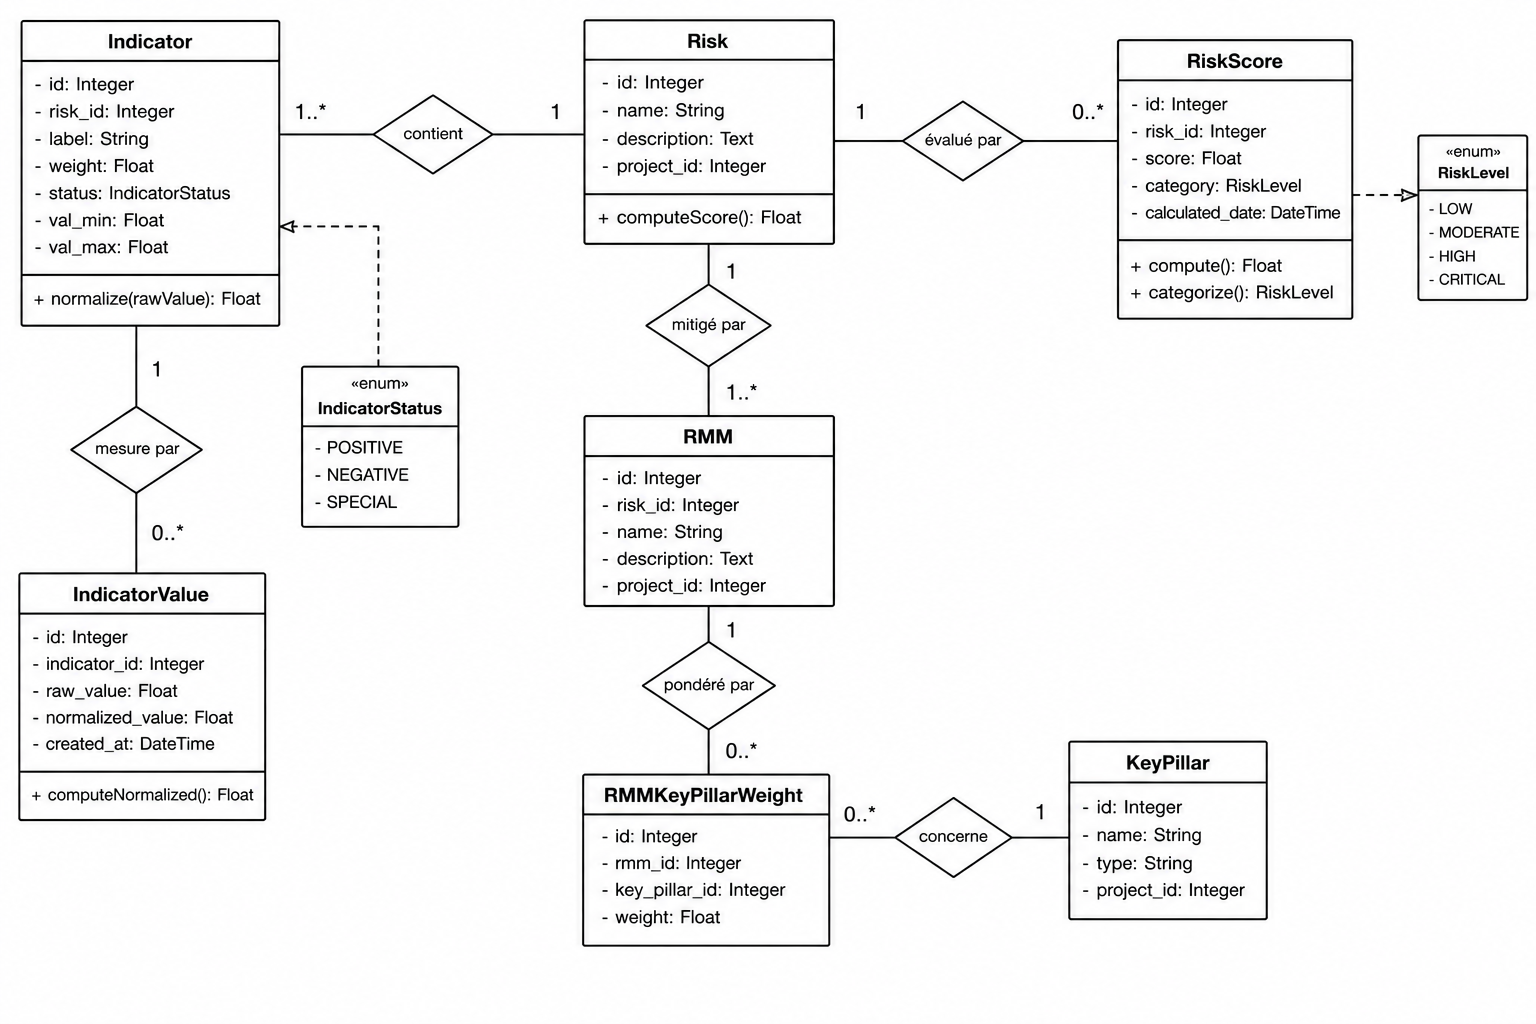
\includegraphics[width=\textwidth]{figures/class_diagram_opage.PNG}
\caption{Diagramme de classes détaillé -- Module O-PAGe}
\end{figure}

Ce diagramme détaille les entités du module O-PAGe dont notre binôme est responsable. Un \textbf{Risk} contient des \textbf{Indicators} dont les valeurs brutes (\textbf{IndicatorValue}) sont normalisées puis agrégées en un \textbf{RiskScore}. Chaque risque est mitigé par des \textbf{RMM} (mécanismes de mitigation) qui sont pondérés par des \textbf{KeyPillars} via \textbf{RMMKeyPillarWeight}.

\subsection{Diagramme de classes -- Administration}

\begin{figure}[H]
\centering
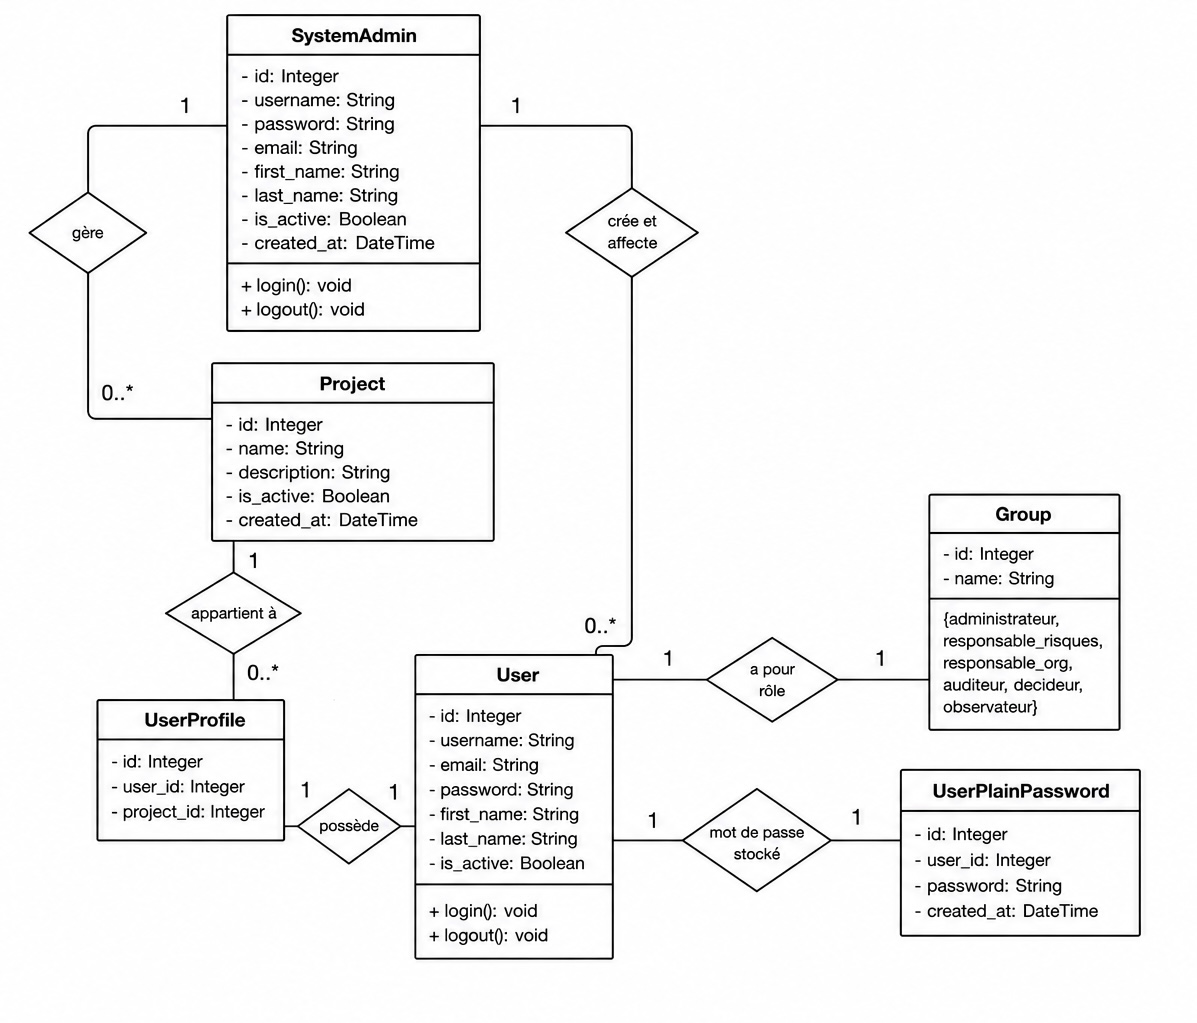
\includegraphics[width=\textwidth]{figures/class_diagram_admin.png}
\caption{Diagramme de classes détaillé -- Administration et gestion des projets}
\end{figure}

Ce diagramme montre l'architecture multi-projets et la gestion des utilisateurs. Le \textbf{SystemAdmin} (modèle séparé avec son propre système d'authentification) gère les \textbf{Projects} (CRUD) et crée les \textbf{Users} en leur affectant un rôle et un projet. Chaque utilisateur possède un \textbf{UserProfile} qui le lie à un projet unique. Le rôle est attribué via un \textbf{Group} (administrateur, responsable\_risques, responsable\_org, auditeur, decideur, observateur). Le mot de passe, généré automatiquement selon le pattern \texttt{\{rôle\}\{numéro\}}, est stocké dans \textbf{UserPlainPassword} pour consultation par l'administrateur.

\section{Architecture technique}

\begin{figure}[H]
\centering
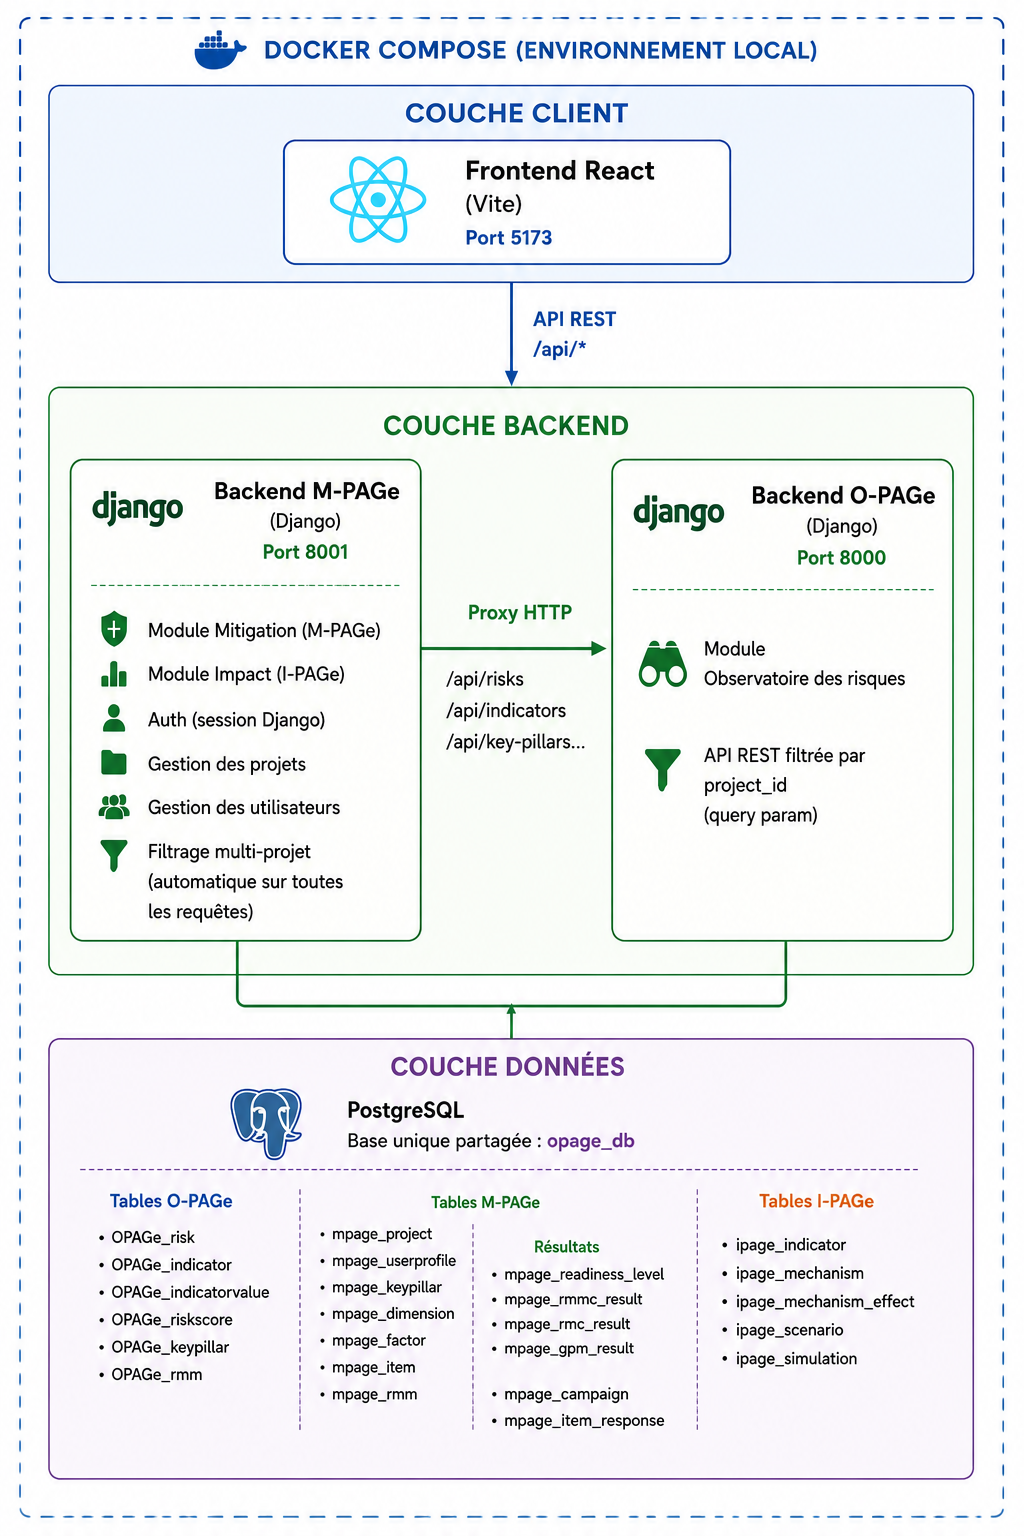
\includegraphics[width=0.8\textwidth]{figures/arch.PNG}
\caption{Architecture technique de la PAGe Platform}
\end{figure}

\begin{itemize}
    \item \textbf{Couche Client} : Frontend React (Vite), port 5173, communique avec le backend M-PAGe via API REST (\texttt{/api/*}).
    \item \textbf{Couche Backend} : deux backends Django :
    \begin{itemize}
        \item \textbf{Backend M-PAGe} (port 8001) : module Mitigation (M-PAGe), module Impact (I-PAGe), authentification (session Django), gestion des projets, gestion des utilisateurs, filtrage multi-projet automatique sur toutes les requêtes.
        \item \textbf{Backend O-PAGe} (port 8000) : module Observatoire des risques, API REST filtrée par \texttt{project\_id} (query param).
    \end{itemize}
    M-PAGe proxie vers O-PAGe via HTTP (\texttt{/api/risks}, \texttt{/api/indicators},\\ \texttt{/api/key-pillars}\ldots).
    \item \textbf{Couche Données} : PostgreSQL, base unique partagée (\texttt{opage\_db}). Les tables sont réparties par module : tables O-PAGe, tables M-PAGe (dont résultats), tables I-PAGe.
    \item \textbf{Conteneurisation} : Docker Compose coordonne l'ensemble des services en environnement local (5 conteneurs : db, opage-backend, mpage-backend, mpage-frontend, pgadmin).
    \item \textbf{Isolation multi-projets} : chaque projet constitue un espace de travail indépendant. Les données (risques, campagnes, mécanismes, simulations) sont isolées par projet via une clé étrangère. Le filtrage est appliqué automatiquement côté backend selon le projet de l'utilisateur connecté.
\end{itemize}

\section{Conclusion}
Ce chapitre a présenté les sept acteurs, les cas d'utilisation par module et ses description, les diagrammes de classes et l'architecture technique. Le chapitre suivant détaille la réalisation.
